%&LaTeX
\documentclass[titlepage,11pt,letterpaper]{article}
\usepackage{float,amsmath,dcolumn,epsfig,ifthen,/Software/latex/vmargin,/Software/latex/harvard_mod}
%\pagestyle{empty}
%&custom12pt

\newcolumntype{d}[1]{D{.}{.}{#1}}
\setmarginsrb{1.2in}{1in}{1.2in}{1.3in}{0pt}{0pt}{0pt}{36pt}
% {left}{top}{right}{bottom}{headheight}{headsep}{footheight}{footskip}

%&custom12pt

\begin{document}

\begin{titlepage}

\hfill{\tiny EpidemiologyOfExp.tex}


\def\thefootnote{\fnsymbol{footnote}}

%\baselineskip=.2in

\enlargethispage{1000pt}
\vspace{0.1in}

\centerline{\LARGE {The Epidemiology of Macroeconomic Expectations}}
\vspace{0.2in}

\centerline{\large Christopher D. Carroll$^{\dagger}$}
\centerline{ccarroll@jhu.edu}
\medskip
\medskip

%\vspace{0.1in}
\begin{table}[H]

%\vspace{.1in}
\centerline{\sc Abstract} 

Since the foundational work of Keynes (1936), macroeconomists have 
emphasized the importance of agents' expectations in determining 
macroeconomic outcomes.  Yet in recent decades macroeconomists have 
devoted almost no effort to modeling actual empirical expectations 
data, instead assuming all agents' expectations are `rational.'  This 
paper takes up the challenge of modeling empirical household 
expectations data, and shows that a simple, standard model from 
epidemiology does a remarkably good job of explaining the deviations 
of household inflation and unemployment expectations from the 
`rational expectations' benchmark.  Furthermore, a microfounded or 
`agent-based' version of the model may be able to explain, in a way 
that still permits aggregation, stark rejections of the pure rational 
expectations framework like Souleles's~\cite{souleles:sentiment} 
finding that members of different demographic groups have sharply 
different predictions for macroeconomic aggregates like the inflation 
rate.


\medskip \medskip {\bf Keywords}: inflation, expectations, unemployment,
monetary policy, agent-based modeling

\medskip
\medskip
{\bf JEL Classification Codes: E0, E3} 

\medskip
\medskip

\small
Subsequent to its original appearance in the form presented here, this
paper was split into two papers.  ``Macroeconomic Expectations of
Households and Professional Forecasters,'' containing the emprical
work and the baseline version of the theoretical model, was published
in the {\it Quarterly Journal of Economics}, Volume 118, Number 1, pp. 
269-298; a paper under the same title as this one, containing the 
more elaborate theoretical work will be published in
{\it The Economy As an Evolving Complex System III}, the proceedings of
a conference at the Santa Fe Institute in November of 2001, in honor
of Kenneth Arrow's contributions to the Santa Fe Institute and to
economics. \medskip

\input titlepage_thanks.tex

\medskip\medskip

The data, econometric programs, and simulation programs that generated 
all of the results in this paper are available on the author's 
website, http://www.econ.jhu.edu/people/carroll.

\medskip\medskip

$^{\dagger}$  Department of Economics, The Johns Hopkins University, Baltimore MD 21218-2685.

\end{table}

\clearpage\pagebreak\vfill\eject

\end{titlepage}
\normalsize
\sloppy 
%\renewcommand{\hbadness}{10000}

\section{Introduction}

%\large \setmarginsrb{0.8in}{0.5in}{0.5in}{0.5in}{0pt}{0pt}{0pt}{0pt}% {left}{top}{right}{bottom}{headheight}{headsep}{footheight}{footskip}\pagestyle{empty}

Ever since the traditional foundation of macroeconomic theory by John
Maynard Keynes~\cite{keynes:generaltheory}, economists have understood
that macroeconomic outcomes depend critically upon expectations about
those outcomes.  Keynes himself believed that in the short run,
economies could experience booms and busts that reflected movements in
the `animal spirits' of business leaders (a view that has some appeal
at the current moment of dot-com hangover), but the basis for most of
today's macro models was laid in the `rational expectations
revolution' of the 1970s.  Led by Lucas, Sargent, Barro, and others,
this approach made a set of assumptions that were much stronger than
rationality alone.  In particular, the framework typically assumes
that all agents in the economy are not merely rational, but also share
identical (correct) beliefs about the structure of the economy, and
have instantaneous and costless access to all the latest economic
data.  Each agent combines these data with the true macroeconomic
model to obtain a forecast for the future path of the economy, on the
assumption that all other agents have identical beliefs and
information (and therefore forecasts).

This set of assumptions has turned out to be a powerful vehicle for 
macroeconomic modeling, but has never been free from the criticism 
that it does not resemble the real world of conflicting opinions and 
forecasts, workers (and even some business leaders) who may not pay 
much attention to macroeconomic matters, and information that can 
sometimes be costly to obtain and process.  Rational expectations 
models also have problems explaining some robust stylized facts, such 
as the apparent inexorability of the tradeoff between inflation and 
unemployment rate (see Ball~\cite{ball:sacrifice} or 
Mankiw~\cite{mankiw:inexorable}).  Despite these problems, the 
rational expectations framework remains the dominant approach in macro 
theory, partly because it tends to be mathematically more tractable 
than alternatives that relax one or another of the framework's 
assumptions.

This paper proposes a tractable alternative framework for the 
formation of a typical person's expectations.  Rather than having their 
own macroeconomic model and constantly feeding it the latest 
statistics, typical people are assumed to obtain their views about the 
future path of the economy from the news media.  Furthermore (and 
importantly), not every person pays close attention to all 
macroeconomic news; instead, people are assumed to absorb the economic 
content of news reports probabilistically, so that it may take quite 
some time for news of changed macroeconomic circumstances to penetrate 
to all agents in the economy.

Roberts~\cite{roberts:inflexp} and Mankiw and 
Reis~\cite{mankiw&reis:stickye} have recently proposed aggregate 
expectations equations that are mathematically very similar to 
aggregate implications of the baseline model derived here.  Roberts's 
work was motivated by his separate findings in 
Roberts~\cite{roberts:phillips,roberts:stickyinfl} that empirical 
macro models perform better in a variety of dimensions when 
survey-based inflation expectations are used in place of constructed 
model-consistent rational expectations.  Mankiw and 
Reis~\cite{mankiw&reis:stickye} obtain similar findings, and 
particularly emphasize the point that these models can explain the 
inexorability of an inflation-unemployment tradeoff much better than 
the standard model with rational expectations does.

However, neither Roberts~\cite{roberts:inflexp} nor Mankiw and 
Reis~\cite{mankiw&reis:stickye} devote much effort to explaining {\it 
why} the dynamics of aggregate expectations should evolve as they 
proposed (though Roberts does suggest that his equation might result 
from the diffusion of press reports).  Mankiw and Reis motivate their 
model by suggesting that there are costs either of obtaining or of 
processing inflation every time an agent updates; however, they do not 
provide an explicit information-costs or processing-costs 
microfoundation.

In contrast, I provide an explicit microfoundation for an aggregate 
expectations equation, grounded in mathematically precise models from 
theoretical epidemiology.  Rather than tracking the spread of a 
disease through a population, the model will track the spread of a 
piece of information (specifically, the information corresponding to 
the latest rational forecast of inflation).

The model's foundation in epidemiology should prove fruitful, both 
because it has novel direct implications of its own, and because the 
rich preexisting literature on more complex models of the spread of 
disease may yield further important and testable 
insights.\footnote{For another example of the application of 
epidemiological models to economics see 
Kremer~\cite{kremer:unionsasdisease}.} For example, taking literally 
the proposition that exposure to news stories is analogous to contact 
with an infectious agent leads to the hypothesis that during periods 
when there is more news coverage of inflation, news should spread 
faster and household expectations should be closer to rational 
expectations.  These predictions are tested and confirmed using an 
index of the intensity of news coverage about inflation.

The paper's final contribution is to relate the model to the 
burgeoning literature on agent-based modeling and social networks that 
has been pioneered, among other places, at the Santa Fe Institute and 
the Center for Social and Economic Dynamics (CSED) at the Brookings 
Institution.  The agent-based modeling approach is useful here for two 
reasons.  First, this approach permits tests of the robustness of the 
baseline model; using agent-based simulations it is straightforward to 
explore a variety of plausible alternative assumptions about the 
spread of information that do not yield the simple analytical equation 
for the dynamics of aggregate expectations obtained for the baseline 
model.  The main finding in these explorations is that the equation 
implied by the baseline model is a good approximation to the dynamics 
of aggregate expectations under several alternative assumptions about 
the information transmission process.  The second advantage of the 
agent-based approach is that it generates agent-level statistics that 
can be compared to the household-level survey data (heretofore mostly 
neglected) from which the aggregate expectations indexes are 
constructed.  As a large literature over the last decade has shown, 
the ability to test aspects of a macro model with micro data can 
enrich both micro and macroeconomics.  Here, I show that the 
qualitative pattern of the changes in the cross-household standard 
deviation of expectations in the data roughly matches the predictions 
of the model (though the level of the standard deviation is greater in 
the data than in the baseline model).


\section{The Epidemiology of Expectations}

% Brief treatment of classical disease in well-mixed population

\subsection{The SIR Model}
Epidemiologists have developed a rich set of models for the 
transmission of disease in a population.  The baseline framework is 
called the Kermack-McKendrick~\cite{kermack&mckendrick:disease} model.  
This model consists of a set of assumptions about who is susceptible 
to the disease, who among the susceptible becomes infected, and 
whether and how individuals recover from the infection (leading to an 
alternate designation as the `SIR' framework).

The standard assumption is that susceptible individual who is exposed 
to the disease in a given period has a fixed probability $p$ of 
catching the disease.  Designating the set of newly infected 
individuals in period $t$ as $N_{t}$ and the set of susceptible 
individuals as $S_{t}$,
\begin{eqnarray}
        N_{t} & = & p S_{t}.
\end{eqnarray}

The next step is to determine susceptibility.  The usual assumption is 
that in order to be susceptible, a healthy individual must have 
contact with an already-infected person.  In a population where each 
individual has an equal probability of encountering any other person 
in the population (a `well-mixed' population), the growth rate of the 
disease will depend upon the fraction of the population already 
infected; if very few individuals are currently infected, the small 
population of diseased people can infect only a small absolute number 
of new victims.

However, there is a special case that is even simpler.  This occurs 
when the disease is not spread person-to-person, but through contact 
with a `common source' of infection.  The classic example is 
Legionnaire's disease, which was transmitted to a group of hotel 
guests via a contaminated air conditioning system (see Fraser et.  
al.~\cite{medline:legionnaires} for a description from the 
epidemiological literature).  Another application is to illness caused 
by common exposure to an environmental factor such as air pollution.  
In these cases, the transmission model is extremely simple: Any 
healthy individual is simply assumed to have a constant probability 
per period of becoming infected from the common source.  This is the 
case we will examine, since below we will assume that news reports 
represent a `common source' of information available to all members of 
the population.

One further assumption is needed to complete the model: The 
probability that someone who is infected will recover from the 
disease.  The simplest possible assumption (which we will use) is that 
infected individuals never recover.

Under this set of assumptions, the dynamics of the disease are as 
follows.  In the first period, proportion $p$ of the population 
catches the disease, leaving $(1-p)$ uninfected.  In period 2, 
proportion $p$ of these people catch the disease, leading to a new 
infection rate of $p(1-p)$ and to a fraction $p+p(1-p)$ of the 
population being infected.  Spinning this process out, it is easy to 
see that starting from period 0 at the beginning of which nobody is 
infected, the total proportion infected at the end of $t$ periods is
\begin{eqnarray}
        \mbox{Fraction Ill} & = & p+p(1-p)+p(1-p)^{2} \ldots + p(1-p)^{t} \label{eq:diseasep} \\
         & = & p \sum_{s=0}^{t} (1-p)^{s} 
\end{eqnarray}
whose limit as $t \rightarrow \infty$ is $p/p=1$, implying that (since 
there is no recovery) everyone will eventually become infected.  In 
the case where `infection' is interpreted as reflecting an agent's 
knowledge of a piece of information, this simply says that eventually 
everyone in the economy will learn a given piece of news.

The last section of the paper explores a richer epidemiological model 
in which diease is spread person-to-person as well as through contact 
with the news media.  And further extensions are possible, and would 
probably prove interesting; as an illustration of some of the 
possibilities, see Kremer~\cite{kremer:unionsasdisease}.


% Legionnaire's disease as a special case where infection rate does
% not depend on population already infected

% Does expectations transmission from person to person change anything?
% Yes, but not much.

\subsection{The Epidemiology of Inflation Expectations}

Now consider a world where most people form their expectations about 
future inflation by reading newspaper articles.  Imagine for the 
moment that every newspaper inflation article contains a complete 
forecast of the inflation rate for all future quarters, and suppose 
(again momentarily) that any person who reads such an article can 
subsequently recall the entire forecast.  Finally, suppose that at any 
point in time $t$ all newspaper articles print identical forecasts.

Assume that not everybody reads every newspaper article on inflation.  
Instead, reading an article on inflation is like becoming infected 
with a common-source disease: In any given period each individual 
faces a constant probability $\lambda$ of becoming `infected' with the 
latest forecast by reading an article.  Individuals who do not 
encounter an inflation article simply continue to believe the last 
forecast they read about.\footnote{This is mathematically very similar 
to the Calvo~\cite{calvoPrices} model in which firms change their 
prices with probability $p$.}

Call $\pi_{t+1}$ the inflation rate between quarter $t$ and quarter $t+1$,
\begin{eqnarray}
        \pi_{t+1} & = & \log(p_{t+1})-\log(p_{t}),
\end{eqnarray}
where $p_{t}$ is the aggregate price index in period $t$.  If we 
define $M_{t}$ as the operator that yields the population-mean value 
of inflation expectations at time $t$ and denote the {\bf N}ewspaper 
forecast printed in quarter $t$ for inflation in quarter $s \geq t$ as 
$N_{t}[\pi_{s}]$, by analogy with equation~\eqref{eq:diseasep} we have 
that
\begin{eqnarray}
        M_{t}[\pi_{t+1}] & = & \lambda N_{t}[\pi_{t+1}]
        +(1-\lambda) \left\{ \lambda N_{t-1}[\pi_{t+1}]
        +(1-\lambda)\left(\lambda N_{t-2}[\pi_{t+1}] 
        + \ldots\right) \right\} \nonumber \\ \label{eq:stickyerat}
\end{eqnarray}

The derivation of this equation is as follows.  In period $t$ a 
fraction $\lambda$ of the population will have been `infected' with 
the current-period newspaper forecast of the inflation rate next 
quarter, $N_{t}[\pi_{t+1}]$.  Fraction $(1-\lambda)$ of the population 
retains the views that they held in period $t-1$ of period $t+1$'s 
inflation rate.  Those period-$t-1$ views in turn can be decomposed 
into a fraction $\lambda$ of people who encountered an article in 
period $t-1$ and obtained the newspaper forecast of period $t+1$'s 
forecast, $N_{t-1}[\pi_{t+1}]$, and a fraction $(1-\lambda)$ who 
retained their period-$t-2$ views about the inflation forecast in 
period $t+1$.  Recursion leads to the remainder of the equation.

This expression for inflation expectations is identical to the one 
proposed by Mankiw and Reis~\cite{mankiw&reis:stickye}.\footnote{It is 
also similar to a formulation estimated by 
Roberts~\cite{roberts:stickyinfl}, except that Roberts uses past 
realizations of the inflation rate rather than past rational 
forecasts.} Mankiw and Reis loosely motivate the equation by arguing 
that developing a full-blown inflation forecast is a costly activity, 
which people might therefore engage in only occasionally.

It is undoubtedly true that developing a reasonably rational 
quarter-by-quarter forecast of the inflation rate arbitrarily far into 
the future would be a very costly enterprise for a typical person (for 
example, it might require obtaining an economics Ph.D. first!).  If 
this were really what people were doing, one might expect them to make 
forecasts only very rarely indeed.

However, reading a newspaper article about inflation, or hearing a 
news story on television or the radio, is not costly in either time or 
money.  There is no reason to suppose that people need to make 
forecasts themselves if news reports provide such forecasts 
essentially for free.  Thus the epidemiological derivation of this 
equation seems considerably more attractive than the loose 
calculation-costs motivation provided by Mankiw and Reis, both because 
this is a fully specified model and because it delivers further 
testable implications (for example, if there is empirical evidence 
that people with higher levels of education are more likely to pay 
attention to news, the model implies that their inflation forecasts 
will on average be closer to the rational forecast; see below for more 
discussion of possible variation in $\lambda$ across population 
groups).

Of course, real newspaper articles do not contain a quarter-by-quarter 
forecast of the inflation rate into the infinite future as assumed in 
the derivation of \eqref{eq:stickyerat}, and even if they did it is 
very unlikely that a typical person would be able to remember the 
detailed pattern of inflation rates far into the future.  In order
to relax these unrealistic assumptions it turns out to be necessary 
to impose some structure on households' implicit views about the
inflation process.

Suppose people believe that at any given time the economy has an 
underlying ``fundamental'' inflation rate.  Furthermore, suppose 
people believe that future changes in the fundamental rate are 
unforecastable; that is, after the next period the fundamental rate 
follows a random walk.  Furthermore, suppose the person believes that 
the actual inflation rate in a given quarter is equal to that period's 
fundamental rate plus an error term $\epsilon_{t}$ which reflects 
unforecastable transitory inflation shocks (reflected in the `special 
factors' that newspaper inflation stories often emphasize).  Thus, the 
person believes that the inflation process is captured by
\begin{eqnarray}
        \pi_{t} & = & \pi_{t}^{f}+\epsilon_{t}            \label{eq:Fpi} 
\\   \pi_{t+1}^{f} & = & \pi_{t}^{f}+\eta_{t+1}  \label{eq:Fpi2}
\\   \pi_{t+2}^{f} & = & \pi_{t+1}^{f}+\eta_{t+2}  \label{eq:Fpi3}
\\ \ldots & & \nonumber
\end{eqnarray}
where $\epsilon_{t}$ is a transitory shock to the inflation rate in 
period $t$ while $\eta_{t}$ is the permanent innovation in the 
fundamental inflation rate in period $t$.  We further assume that 
consumers believe that values of $\eta$ beyond period $t+1$, and 
values of $\epsilon$ beyond period $t$, are unforecastable white noise 
variables; that is, future changes in the fundamental inflation rate 
are unforecastable, and transitory shocks are expected to go 
away.\footnote{Note that we are allowing people to have some idea 
about how next quarter's fundamental rate may differ from the current 
quarter's rate, because we did not impose that consumers' expectations 
of $\eta_{t+1}$ must equal zero.}

Before proceeding it is worth considering whether this is a plausible 
view of the inflation process; we would not want to build a model on 
an assumption that people believe something patently absurd.  
Certainly, it would not be plausible to suppose that people always and 
everywhere belive that the inflation rate is characterized 
by~\eqref{eq:Fpi}-\eqref{eq:Fpi3}; for example, 
Ball~\cite{ball:nearrational} shows that in the US from 1879-1914 the 
inflation rate was not persistent in the US, while in other countries 
there have been episodes of hyperinflation (and rapid disinflation) in 
which views like~\eqref{eq:Fpi}-\eqref{eq:Fpi3} would have been 
nonsense.

However, the relevant question for the purposes of this paper is 
whether this view of the inflation process is plausible for the period 
for which I have inflation expectations data.  Perhaps the best way to 
examine this is to ask whether the univariate statistical process for 
the inflation rate implied by \eqref{eq:Fpi} and \eqref{eq:Fpi2} is 
strongly at odds with the actual univariate inflation process.  In 
other words, after allowing for transitory shocks, does the inflation 
rate approximately follow a random walk?

\input DataAndPrograms/Volumes/Data/ADFpi.tex

The appropriate statistical test is an augmented Dickey-Fuller test.  
Table~\ref{table:ADFpi} presents the results from such a test.  The 
second row shows that even with more than 160 quarters of data it is 
not possible to reject at a 5 percent significance level the 
proposition that the core inflation rate follows a random walk with a 
one-period transitory component - that is, it is not possible to 
reject the process defined 
by~\eqref{eq:Fpi}-\eqref{eq:Fpi3}.\footnote{The near-unit-root feature 
of the inflation rate in the post-1959 period is well known to 
inflation researchers; some authors find that a unit root can be 
rejected for some measures of inflation over some time periods, but it 
seems fair to say that the conventional wisdom is that at least since 
the late 1950s inflation is `close' to a unit root process.  See 
Barsky~\cite{barsky:fisher} for a more complete analysis, or 
Ball~\cite{ball:nearrational} for a more recent treatment.} When the 
transitory shock is allowed to have effects that last for two quarters 
rather than one, it is not possible to reject a random walk in the 
fundamental component even at the 10 percent level of significance 
(the last row in the table).

Note that the unit root (or near unit root) in inflation does not 
imply that future inflation rates are totally unpredictable, only that 
the history of inflation by itself is not very useful in forecasting 
future inflation {\it changes} (beyond the disappearance of the 
transitory component of the current period's shock).  This does not 
exclude the possibility that current and lagged values of other 
variables might have predictive power.  Thus, this view of the 
inflation rate is not necessarily in conflict with the vast and 
venerable literature showing that other variables (most notably the 
unemployment rate) do have considerable predictive power for the 
inflation rate (see Staiger, Stock, and Watson~\cite{ssw:nairu} for a 
recent treatment).

Suppose now that rather than containing a forecast for the entire 
quarter-by-quarter future history of the inflation rate, newspaper 
articles simply contain a forecast of the inflation rate over the next 
year.  This is not an implausible assumption; newspaper articles on 
inflation (which are usually published the day after inflation 
statistics are released) often contain interviews with expert 
forecasters, who are frequently asked for their forecasts of future 
inflation rates.  The most common such forecast is for the inflation 
rate over the next year.  It is not implausible, therefore, to suppose 
that at least part of what readers take away from such stories is a 
sense of what to expect for the average inflation rate over the next 
year.

The next step is to figure out how such a one-year forecast for 
inflation can be integrated into some modified version of 
equation~\eqref{eq:stickyerat}.  To capture this, we must introduce a 
bit more notation.  Define $\pi_{s,t}$ as the inflation rate between 
periods $s$ and $t$, converted to an annual rate.  Thus, for example, 
in quarterly data we can define the inflation rate for quarter $t+1$ 
at an annual rate as
\begin{eqnarray}
        \pi_{t,t+1} & = & 4 (\log p_{t+1} - \log p_{t})
\\  & = & 4 \pi_{t+1}   
\end{eqnarray}
where the factor of four is required to convert the quarterly price 
change to an annual rate.

Our hypothetical person's view is that the true {\it ex-post} 
inflation rate over the next year will be given by
\begin{eqnarray}
    \pi_{t,t+4} & = & \pi_{t+1}+\pi_{t+2}+\pi_{t+3}+\pi_{t+4} 
\\   & = & \pi_{t+1}^{f}+\epsilon_{t+1}+\pi_{t+2}^{f}+\epsilon_{t+2}+\pi_{t+3}^{f}+\epsilon_{t+3}+\pi_{t+4}^{f}+\epsilon_{t+4}
\\   & = & \pi_{t+1}^{f}+\epsilon_{t+1}+\pi_{t+1}^{f}+\eta_{t+2}+\epsilon_{t+2}+\pi_{t+1}^{f}+\eta_{t+2}+\eta_{t+3}+\epsilon_{t+3}+ \nonumber
\\   & & \pi_{t+1}^{f}+\eta_{t+2}+\eta_{t+3}+\eta_{t+4}+\epsilon_{t+4}.  \label{eq:pittp4}
\end{eqnarray}

To proceed, it will be necessary to consider people's expectations 
about future inflation rates.  Define $F_{t}[\bullet_{s}]$ as the 
agent's forecast (expectation) as of date $t$ of $\bullet_{s}$, for an 
agent who updates his views from a news report in period $t$.  Using 
this notation, the assumptions we made earlier about the stochastic 
processes for $\epsilon$ and $\eta$ imply that 
$F_{t}[\epsilon_{t+n}]=F_{t}[\eta_{t+n+1}]=0$ for all $n>0$.

Applying the $F_{t}$ operator to both sides of~\eqref{eq:pittp4}
implies that the person's forecast of the inflation rate over the
next year is simply equal to four times his forecast of the fundamental inflation
rate for next quarter:
\begin{eqnarray}
    F_{t}[\pi_{t,t+4}] & = & 4 F_{t}[\pi_{t+1}^{f} ]
\\  & = & F_{t}[\pi_{t,t+1}^{f}]    
%\\  & = & F_{t}[\pi_{t,t+1}]    
\end{eqnarray}

Now for an important conclusion: If people believe that the forecasts 
printed in the newspaper also embody the same view of the inflation 
process embodied in~\eqref{eq:Fpi}-\eqref{eq:Fpi3}, then an identical 
analysis leads to the conclusion that (defining the `newspaper 
expectations' operator $N_{t}$ similarly to the consumer's 
expectations operator):
\begin{eqnarray}
    N_{t}[\pi_{t,t+4}] & = & 4 N_{t}[\pi_{t+1}^{f} ]
\\  & = & N_{t}[\pi_{t,t+1}^{f}]    
%\\  & = & N_{t}[\pi_{t,t+1}]    
\end{eqnarray}

Thus, the newspaper forecast contains only a single important piece of 
information about the future: a projection of the fundamental 
inflation rate over the next year, which the unit root theory implies 
is the expected fundamental rate in all of the year's constituent 
quarters and all subsequent quarters as well.  A consumer who reads 
the newspaper in period $t$, therefore, will update his expectations 
to equal the corresponding newspaper forecasts:
\begin{eqnarray}
    F_{t}[\pi_{t,t+1}] =  F_{t}[\pi_{t,t+4}] = F_{t}[\pi_{t,t+4}^{f}] & = & N_{t}[\pi_{t,t+4}^{f} ] = N_{t}[\pi_{t,t+4}].
%\\  F_{t}[\pi_{t+1}] & = & N_{t}[\pi_{t+1}].
\end{eqnarray}

The rightmost equality holds because the consumer assumes the 
newspaper has no information about $\epsilon_{t+n}$ or $\eta_{t+n+1}$, 
so for $n>0$, $N_{t}[\epsilon_{t+n}]=N_{t}[\eta_{t+n+1}]=0$.  The next 
equality to the left holds because we assume that when the consumer 
reads the newspaper his views are updated to the views printed in the 
newspaper.  The other two equalities similarly hold because 
$F_{t}[\epsilon_{t+n}]=F_{t}[\eta_{t+n+1}]=0$.

Now note a crucial point: the assumption that changes in the inflation
rate beyond period $t+1$ are unforecastable means that 
\begin{eqnarray}
        F_{t-1}[\pi_{t-1,t+3}] & = & F_{t-1}[\pi_{t,t+4}] \label{eq:ftm1} \\
        F_{t-2}[\pi_{t-2,t+2}] & = & F_{t-2}[\pi_{t,t+4}] \label{eq:ftm2} \\ 
        \ldots & & \label{eq:ftmn}
\end{eqnarray}

Now note that an equation similar to \eqref{eq:stickyerat} can 
be written for projections of the inflation rate over the
next year:
\begin{eqnarray}
        M_{t}[\pi_{t,t+4}] & = & \lambda F_{t}[\pi_{t,t+4}]
        +(1-\lambda) \left\{ \lambda F_{t-1}[\pi_{t,t+4}]
        +(1-\lambda)\left(\lambda F_{t-2}[\pi_{t,t+4}] 
        + \ldots\right) \right\} \nonumber,
\end{eqnarray}
and substituting~\eqref{eq:ftm1}-\eqref{eq:ftmn} into this equation
and replacing $F_{t}$ with $N_{t}$ on the assumption that the newspaper
forecasts are the source of updating information, we obtain
\begin{eqnarray}
        M_{t}[\pi_{t,t+4}] & = & \lambda F_{t}[\pi_{t,t+4}]
        +(1-\lambda) \left\{ \lambda F_{t-1}[\pi_{t-1,t+3}]
        +(1-\lambda)\left(\lambda F_{t-2}[\pi_{t-2,t+2}] 
        + \ldots\right) \right\} \nonumber \\ 
        M_{t}[\pi_{t,t+4}] & = & \lambda F_{t}[\pi_{t,t+4}]
        +(1-\lambda) M_{t-1}[\pi_{t-1,t+3}] \\
        M_{t}[\pi_{t,t+4}] & = & \lambda N_{t}[\pi_{t,t+4}]
        +(1-\lambda) M_{t-1}[\pi_{t-1,t+3}]. \label{eq:esteqn}
\end{eqnarray}

That is, mean measured inflation expectations for the next year should 
be a weighted average between the current `rational' (or newspaper) 
forecast and last period's mean measured inflation expectations.  This 
equation is therefore directly estimable, assuming an appropriate 
proxy for newspaper expectations can be constructed.\footnote{This 
equation is basically the same as equation (5) in 
Roberts~\cite{roberts:inflexp}, except that Roberts proposes that the 
forecast toward which household expectations are moving is the 
`mathematically rational' forecast (and he simply proposes the 
equation without examining the underlying logic that might produce 
it).}

Readers uncomfortable with the strong assumptions needed to 
derive~\eqref{eq:esteqn} may be happier upon noting that the equation
\begin{eqnarray}
 M_{t}[\pi_{t,t+4}] & = & \lambda N_{t}[\pi_{t,t+4}] + (1-\lambda) M_{t-1}[\pi_{t,t+4}] \label{eq:pinoapprox}
\end{eqnarray}
can be derived without any assumptions on consumers' beliefs about the 
inflation process; the difference between~\eqref{eq:esteqn} and 
\eqref{eq:pinoapprox} is only in the subscript on the $\pi$ term 
inside the $M_{t-1}$ operator.  The assumptions made above were those 
necessary to rigorously obtain $M_{t-1}[\pi_{t,t+4}] = 
M_{t-1}[\pi_{t-1,t+3}]$.  In practice, however, even a much more 
realistic view of the inflation process would likely imply a very high 
degree of correlation between the period-$t-1$ projection of the 
inflation rate over the year beginning in quarter $t$ and the 
period-$t-1$ projection of the inflation rate over the year beginning 
in quarter $t+1$.  Indeed, three of out of the four quarters ($t+2, 
t+3, $ and $t+4$) are identical between the two projections; the only 
differences between the two measures would have to spring from the 
consumer's projection of the difference between the inflation rates in 
quarters $t+1$ and $t+5$.

\section{Estimation}

Estimating equation~\eqref{eq:esteqn} requires us to identify data 
sources for population-mean inflation expectations and for `newspaper' 
forecasts of inflation over the next year.

The University of Michigan conducts a monthly survey of households 
that is intended to be representative of the population of the United 
States.  One component of the survey asks households what they expect 
the inflation rate to be over the next year (for details on the exact 
questions, and the controls for question validity, see 
Curtin~\cite{curtin:inflsurvart}).  I will directly use the mean 
inflation forecast from this survey as my proxy for 
$M_{t}[\pi_{t,t+4}]$.

Identifying the `newspaper' forecast for next-quarter inflation might 
seem more problematic, but there is a surprisingly good candidate: The 
median four-quarter inflation forecast from the Survey of Professional 
Forecasters (henceforth, SPF).  The SPF, currently conducted by the 
Federal Reserve Bank of Philadelphia and previously a joint product of 
the National Bureau of Economic Research and the American Statistical 
Association, has collected and summarized forecasts from leading 
private forecasting firms since 1968.  The survey instrument is 
distributed once a quarter, just after the middle of the second month 
of the quarter, and responses are due within a couple of weeks.  The 
survey asks participants for quarter-by-quarter forecasts, spanning 
the current and next 5 quarters, for a wide variety of economic 
variables, including GDP growth, various measures of inflation 
including CPI inflation, and the unemployment rate.  For more details 
on the SPF, see Croushore~\cite{croushore:introSPF}.

As noted above, the typical newspaper article on inflation interviews 
some `experts' on inflation.  The obvious candidates for such experts 
are the set of people who forecast the economy for a living, so the 
pool of interviewees is likely to be approximately the same group of 
forecasters whose views are summarized by the SPF. Hence, it seems 
reasonable to identify $N_{t}$ with the SPF inflation expectations 
data.

\subsection{Do the Forecasts Forecast?}

There is a substantial existing literature on the forecasting 
performance of various survey measures of inflation expectations 
including the Michigan Survey and the SPF. Early papers 
(Turnovsky~\cite{turnovsky:inflsurv}, Bryan and 
Gavin~\cite{bryan&gavin:inflsurv}) claimed to find statistically 
significant biases in some survey measures of expected inflation, but 
a recent review paper by Croushore~\cite{croushore:spfisgood} shows 
that some of those results were spurious (due to improper treatment of 
the data or econometric problems), and that none of the results hold 
up when the sample period is updated to include data for the last 10 
or 15 years.  Croushore specifically examines both the Michigan survey 
and the SPF, and finds no evidence of bias over the entire sample for 
either survey.  In most respects he finds the SPF a better forecaster 
of inflation outcomes than the Michigan 
survey.\footnote{Unfortunately, the well-known recent survey paper by 
Thomas~\cite{thomas:surveyinfl} largely neglects the SPF, and focuses 
instead mainly on comparisons of the Michigan survey and the 
Livingston survey.  Thomas finds the median of the Michigan survey to 
be a better forecaster than the mean, but my model delivers 
predictions only for the mean and not for the median, so I neglect the 
Michigan median in my empirical work.  See the appendix to 
Roberts~\cite{roberts:stickyinfl} for more evidence on the 
inefficiency of the Michigan survey.}

For the purposes of this paper, there are two important `sniff-test' 
questions that should be addressed before attempting formal estimation 
of the model \eqref{eq:esteqn}.  First, do both the Michigan and SPF 
survey measures of inflation expectations have statistically 
significant ability to predict future inflation?  And, second, is the 
SPF forecast better in some sense than the Michigan forecast, as 
assumed in the model?

As a first step, consider the implications of the statistical test 
performed in Table~\ref{table:ADFpi}, which was unable to reject the 
hypothesis that inflation has a unit root.  The high serial 
correlation in the inflation rate discovered by the unit root test 
means that future levels of the inflation rate will be highly 
predictable based on the recent past history of inflation.  The 
interesting question is therefore whether the survey forecasts have 
predictive power for the future inflation rate {\it beyond} what could 
be predicted based on past inflation data.

\input DataAndPrograms/Volumes/Data/piforc.tex


To answer this question, Table~\ref{table:piforc} presents a 
regression of the actual inflation rate over the next year on the 
Michigan and SPF measures of expected inflation, along with the most 
recent annual inflation statistic available at the time the SPF and 
Michigan forecasts were made.  Both measures have highly statistically 
significant predictive power for future inflation even controlling for 
the inflation rate's recent past history, but the SPF measure has 
substantially more predictive power.\footnote{Actually, quarter 
$t-1$'s inflation rate is included among the regressors even though it 
is not known until about the middle of the first month of quarter $t$, 
so about a sixth of the people whose views are summarized in the 
Michgian survey cannot have known $\pi_{t-1}$.  This makes it harder 
for the Michigan survey to be statistically significant because the 
lagged inflation statistic has an unfair advantage since it 
incorporates information some surveyed people could not have known; the 
survey is significant despite this handicap.  This issue does not 
arise with the SPF forecast because $\pi_{t-1}$ has been reported by 
the time the SPF survey is conducted.} Both measures of inflation 
expectations remain highly statistically significant even controlling 
for previously known inflation rates, and the `horserace' regression 
results indicate that the Michigan survey measure contains no 
information that is not also included in the SPF measure, while the 
SPF forecast has highly statistically significant predictive power 
that is not contained in the Michigan survey.\footnote{Technical 
considerations suggest that it might be more appropriate to include 
several lags of quarterly inflation rates as the control variables for 
past inflation rates in the regressions reported in 
table~\ref{table:piforc}.  When this is done the results remain 
substantially the same.  Results for the annual inflation rate are 
reported because they are less cumbersome to present.  Quarterly 
results are available from the author, or can be generated by running 
the set of RATS programs available on the author's web page that 
generated all empirical results in this paper.}

An alternative, and more stringent, test of the predictive power of 
the surveys is whether they can predict the {\it change} in the 
inflation rate.  Under the assumption that the fundamental inflation 
rate follows the unit root process outlined in equations 
\eqref{eq:Fpi} to \eqref{eq:Fpi3} (which was consistent with the 
empirical tests from Table~\ref{table:ADFpi}), the difference between 
the inflation rate over the coming year and the most recently 
published quarterly inflation statistic is (cf. \eqref{eq:pittp4})
\begin{eqnarray}
        \pi_{t,t+4} - \pi_{t-2,t-1} & = & \phantom{-}4 \phantom{(} F_{t\phantom{-1}}[\pi_{t}]+4\eta_{t+1}+3 \eta_{t+2}+2\eta_{t+3}+\eta_{t+4}+\epsilon_{t+1}+\epsilon_{t+2}+\epsilon_{t+3}+\epsilon_{t+4} \nonumber 
\\  &   &        - 4 (F_{t-1}[\pi_{t-1}]+\epsilon_{t-1}) \nonumber
\\  & = & 4 \eta_{t}+4\eta_{t+1}+3 \eta_{t+2}+2\eta_{t+3}+\eta_{t+4} \nonumber
\\  &   & +\epsilon_{t+1}+\epsilon_{t+2}+\epsilon_{t+3}+\epsilon_{t+4} - 4 \epsilon_{t} -4 \epsilon_{t-1} \nonumber 
\end{eqnarray}

Earlier we assumed that people believe that professional forecasters 
have some knowledge of $\epsilon_{t}$, $\eta_{t}$, and $\eta_{t+1}$, 
so even under the assumption that the inflation process has a unit 
root this equation tells us that there should be a substantial 
component of predictability in the change in the inflation rate.  
Furthermore, we have thus far made no assumptions about what the 
professional forecasters actually know about the future; for example, 
they may use the unemployment rate to forecast changes in inflation.  
Thus, there is even more scope for the SPF than for the Michigan 
survey to predict changes in the inflation rate.

Results from regressions of $\pi_{t,t+4}-\pi_{t-2,t-1}$ on the two 
survey forecasts of inflation are presented in the next three rows of 
table~\ref{table:piforc}.  Again, both survey measures have highly 
statistically significant explanatory power for the change in the 
inflation rate, and again the SPF forecast wins the horserace by a big 
margin.\footnote{Similar results are obtained when last quarter's 
inflation rate is replaced by the inflation rate over the year leading 
up to the previous quarter.}

In sum, all these results are qualitatively what would be expected 
from the model as described above: the forecast from the survey of 
households has significant predictive power for future inflation, but 
the SPF forecast has much more power.

Of course, a finding that the SPF forecast is better than the Michigan 
forecast does not necessarily imply that the SPF forecast is fully 
rational.  It remains possible that inflation forecasts could have 
been constructed that were even better than those of the SPF. However, 
Croushore~\cite{croushore:spfisgood} shows that it would have been 
difficult to improve upon the SPF forecasts using information that was 
available at the time the SPF forecasts were made.\footnote{Croushore 
points out an important flaw in previous studies of the rationality of 
forecasts; previous authors regressed inflation outcomes on 
information that was available at the time the SPF forecasts were 
made, and concluded that any finding of statistical significance 
indicated a failure of rationality.  But such a test implicitly 
assumes that rationality means that forecasters should have known in 
advance not just that a data realization had occurred, but also the 
effects that that realization should have on future inflation rates.  For 
example, it supposes that `rational' forecasters in 1973 would have 
known the precise effects oil shocks would have on subsequent 
inflation rates.  But no similar experience existed upon which 
forecasters could base their forecasts, so finding {\it ex post} that 
an oil shock variable is statistically significant does not imply that 
forecasters were irrational not to have predicted its effects {\it ex 
ante}.} Furthermore, from the standpoint of the model the appropriate 
measure of $N_{t}[\pi_{t,t+1}]$ is what people might actually be able 
to read about in a newspaper or hear about in a news report on 
television.  Since the Survey of Professional Forecasters is designed 
to incorporate forecasts from the leading macroeconomic forecasters in 
each period, it is likely that the economists who are contacted by 
journalists writing about inflation will be the same people 
contributing their forecasts to the SPF. If this is true, the SPF 
forecast would be the right one to use for our purposes even if there 
were systematic biases in its forecasts.

\subsection{Estimating the Stickiness of Inflation Expectations}

We can now turn to the main question, which is whether the Michigan 
forecast can be reasonably well represented as a distributed lag of 
the SPF forecast; that is, whether \eqref{eq:esteqn} provides a good 
empirical description of the dynamics of the Michigan survey's measure 
of household inflation expectations.

\input DataAndPrograms/Volumes/Data/esteqn.tex

To provide a baseline for comparison, the first line of 
Table~\ref{table:esteqn} presents results for the simplest possible 
model: that the value of the Michigan index of inflation expectations 
$M_{t}[\pi_{t,t+4}]$ is equal to a constant, $\alpha_{0}$.  By 
definition the $\bar{R}^{2}$ is equal to zero; the standard error of 
the estimate is 0.88.  The last column of the table is reserved 
for reporting the results of various tests that will be conducted as 
the analysis progresses.  By way of example, the test performed for 
the benchmark expectations-constant model is whether the average value 
of the expectations index is zero, $\alpha_{0} = 0$.  Unsurprisingly, 
this nonsensical proposition can be rejected with an overwhelming 
degree of statistical confidence, as indicated by a $p$-value that 
says that the probability that the proposition is true is zero.

We begin to examine the baseline model's ability to explain the Michigan
data by estimating
\begin{eqnarray}
        M_{t}[\pi_{t,t+4}] & = & \alpha_{1}S_{t}[\pi_{t,t+4}]+\alpha_{2}M_{t}[\pi_{t-1,t+3}]+\nu_{t}, \label{eq:firstest}
\end{eqnarray} 
where $S_{t}[\pi_{t,t+4}]$ is the corresponding SPF forecast.  
Comparing this to \eqref{eq:esteqn} provides the testable restriction 
that $\alpha_{2}=1-\alpha_{1}$ or, equivalently,
\begin{equation}
\alpha_{1}+\alpha_{2}=1 \label{eq:restriction}.
\end{equation}

Results from the estimation of \eqref{eq:firstest} are presented as 
equation 1 in Table~\ref{table:esteqn}.  The point estimates of 
$\alpha_{1}=0.36$ and $\alpha_{2}=0.66$ suggest that the restriction 
\eqref{eq:restriction} is very close to holding true, and the last 
column presents formal statistical evidence on the question: It shows 
the statistical significance with which the proposition that 
$\alpha_{1}+\alpha_{2}=1$ can be rejected.  The p-value indicates that 
the restriction is easily accommodated by the data at the conventional 
level of significance of 0.05 or greater.  Estimation results when the 
restriction is imposed in estimation are presented in the next row of 
the table, which provides our first unambiguous estimate of the 
crucial coefficient: $\lambda= 0.27$.  Note that the Durbin-Watson 
statistic indicates that there is no evidence of serial correlation in 
the residuals of the equation (a Q-test yields the same result), which 
is impressive because the individual series involved have very high 
degrees of serial correlation (cf.  the unit root tests in 
table~\ref{table:ADFpi} and the Durbin-Watson statistics in 
table~\ref{table:piforc}).  This is evidence that the two variables 
are cointegrated, as would be expected if one were a distributed lag 
of the other.

The point estimate $\lambda=0.27$ is remarkably close to the value of 
$0.25$ assumed by Mankiw and Reis~\cite{mankiw&reis:stickye} in their 
simulation experiments; unsurprisingly, the last column for equation 2 
indicates that the proposition $\alpha_{1}=\lambda=0.25$ is easily 
accepted by the data.  This indicates that in each quarter, only about 
one fourth of households have a completely up-to-date forecast of the 
inflation rate over the coming year.  On the other hand, this estimate 
also indicates that only about 32 percent ($=(1-0.25)^{4})$ of 
households have inflation expectations that are more than a year out 
of date.

As noted above, Roberts~\cite{roberts:inflexp} estimated a similar 
equation, except that his proposal was that expectations move toward 
the mathematically rational forecast of inflation.  Since such a 
forecast is unobservable, he used the actual inflation rate and 
instrumented using a set of predetermined instruments, on the usual 
view that if the instruments are valid the estimation should yield an 
unbiased estimate of the coefficient on the true but unobservable 
rational forecast.  However, this procedure is problematic if there 
was anything that the `rational' forecaster did not know about the 
structure of the economy and had to learn from realizations over time; 
as Roberts acknowledges, it is also problematic if the structure of 
the economy changes over time.  A further drawback to this approach is 
that instrumenting can cause a severe loss of efficiency.  Since the 
theory proposed here is quite literally that household expectations 
move toward the SPF forecast, there is no reason to instrument.  In 
the end, however, Roberts's parameter estimates are similar to those 
obtained here, though considerably less precise.

Intutitively it might seem that if almost 70 percent of agents have 
inflation expectations that are of a vintage of a year or less, the 
behavior of the macroeconomy could not be all that different from what 
would be expected if all expectations were completely up-to-date.  The 
surprising message of 
Roberts~\cite{roberts:stickyinfl,roberts:phillips} and Mankiw and 
Reis~\cite{mankiw&reis:stickye} is that this intuition is wrong.  
Mankiw and Reis show that an economy with $\lambda=0.25$ behaves in 
ways that are sharply different from an economy with fully rational 
expectations ($\lambda=1$), and argue that in each case where behavior 
is different the behavior of the $\lambda=0.25$ economy corresponds 
better with empirical evidence (for example with respect to the effect 
of interest rate shocks on aggregate output).

Mankiw and Reis~\cite{mankiw&reis:stickye} simply postulated 
$\lambda=0.25$.  What equation 2 of Table~\ref{table:esteqn} indicates 
is that if the data are forced to choose a $\lambda$ they are happy 
with that choice.  However, we have not allowed the data to speak to 
the question of whether there is a better representation of inflation 
expectations than \eqref{eq:firstest}.

The first avenue by which we might wish to let the data reject the 
specification is to allow a constant into the equation.  Equation 3 of 
table~\ref{table:esteqn} presents the results.  The last column 
indicates that the proposition that the constant term is zero can be 
rejected at a very high level of statistical significance; the data do 
indeed want a constant in the regression equation.  On the other hand, 
the improvement in fit that comes with a constant is rather modest: 
the standard error declines from about 0.43 without the constant to 
about 0.35 with it.  Compared with a standard deviation for the 
dependent variable of about 0.88, this improvement in fit is not very 
impressive, even if it is statistically significant.

Furthermore, if the model is to be treated as a structural description 
of the true process by which inflation expectations are formed, the 
presence of a constant term does not make much sense.  It implies, for 
example, that if both actual inflation and the rational forecast for 
inflation were to go to zero forever, people would continue to believe 
in a positive inflation rate (of about 2 percent) forever.  It seems 
much more likely that under these circumstances people would 
eventually learn to expect an inflation rate of zero.  This point can 
be generalized to show that if the actual inflation rate and the 
rational forecast were fixed forever at {\it any} constant value, 
people's expectations would never converge to the true, constant 
inflation rate, but instead would be perpetually biased unless the 
true value happened to be exactly equal to the single stable point of 
the estimated equation.  (See the final section of the paper for a 
demonstration that the presence of a significant constant term could 
reflect the presence of some social transmission of inflation 
expectations via conversations with neighbors, in addition to the 
news-media channel examined here).

A modification to the model that makes more sense than a constant term 
is to allow for the possibility that some people update their view of 
the fundamental inflation rate to the most recent {\it past} inflation 
rate rather than to the SPF forecast of the future inflation rate.  
Indeed, since most news coverage of inflation is prompted by the 
release of the most recent past inflation statistics (and since the 
new number is often in the headline of the news article) one might 
argue that it would be {\it more} likely for people to update their 
expectations to the past inflation rate than to a forecast of the 
future rate.

We can examine this possibility by estimating an equation of the form
\begin{eqnarray}
        M_{t}[\pi_{t,t+4}] & = & \alpha_{1} S_{t}[\pi_{t,t+4}]+\alpha_{2} M_{t-1}[\pi_{t-1,t+3}]+\alpha_{3} P_{t}[\pi_{t-5,t-1}].
\end{eqnarray}
where $P_{t}[\pi_{t-5,t-1}]$ represents the most recently published 
annual inflation rate as of time $t$.

In the epidemiological sense, derivations similar to those provided 
above for the baseline model can be performed to show that this 
equation can be interpreted as representing a model in which there are 
two competing sources of `infection,' the forecast of the future 
inflation rate and the actual past inflation rate.  A given person's 
view of the fundamental inflation rate may come from either of these 
two sources, but a given person can be infected from only one of these 
sources at a time.

Results from estimating this equation are presented in the next row of 
Table~\ref{table:esteqn}.  The past inflation rate is indeed highly 
statistically significant - but with a {\it negative} coefficient!  
The negative coefficient makes no sense, as it implies that a higher 
past inflation rate convinces people that the fundamental inflation 
rate is lower.  The final row of the table, however, shows that when a 
constant is included in this regression, the past inflation rate is no 
longer statistically significant, while the forecast of the future 
inflation rate remains highly statistically significant.  This seems 
to indicate that the significance of the past inflation rate is 
spurious, in the sense that the past inflation rate is just proxying 
for the missing constant term, which we have already acknowledged to 
be statistically significant.  The last row in the table shows, 
surprisingly, that even when the SPF forecast is entirely absent, the 
lagged inflation rate has no explanatory power for the Michigan survey 
after controlling for the lagged value of the survey; furthermore, the 
Durbin-Watson suggests a substantial amount of negative serial 
correlation in the residuals of this equation.

In sum, it seems fair to say that the simple `sticky expectations' 
equation~\eqref{eq:esteqn} does a remarkably good job of capturing 
much of the predictable behavior of the Michigan inflation 
expectations index.

\subsection{Timing Issues: Monthly vs Quarterly, Michigan vs SPF}

However, there is a potential problem.  If we want to take our model's 
updating equation~\eqref{eq:esteqn} seriously as reflecting the effect 
of news reports on people's perceptions, it is logically necessary for 
the news reports to have been published before people's expectations 
can move toward them.  This obvious point raises some conceptual 
difficulties about the empirical results presented thus far, because 
the actual timing of the quarterly Michigan and SPF surveys does not 
match up with the implied time structure in the model we have 
presented and estimated.

Most newspaper stories on inflation appear the day after the monthly 
release of inflation statistics, which happens around mid-month every 
month.  Between mid-month and the beginning of the next month, there 
are typically few economic statistics released that would have much 
impact on a rational forecast of the inflation rate.  Given these 
facts, if the Michigan survey for month $t+1$ were conducted entirely 
on the first day of month $t+1$, there would be little reason to 
object to an updating equation of the form
\begin{eqnarray}
M_{t+1}[\pi_{t+1,t+13}] & = & \lambda N_{t}[\pi_{t,t+12}] + (1-\lambda) M_{t}[\pi_{t,t+12}],  \label{eq:monthlym3}
\end{eqnarray}
where $N_{t}$ designates the inflation forecast embodied in the 
typical newspaper article published in the middle of month $t$.

Now consider the circumstances under which it would be appropriate to 
proxy the newspaper forecasts $N_{t}$ with the Survey of Professional 
Forecasters' forecast $S_{t}$.  The SPF is conducted once a quarter, 
during the quarter's middle month.  Forecasts are collected beginning 
right after the inflation data for the previous month are reported, 
which is exactly the time that most news articles on inflation are 
being written; although survey participants have a week or so to turn 
in their forecasts, typically little or no important economic data are 
released before the survey deadline, so there is little reason to 
expect the views reflected in the SPF to be much different from the 
views the news media will have reported in mid-month.  Hence, if month 
$t$ was an SPF survey month there would be little reason to object to 
proxying $N_{t}$ with $S_{t}$ in \eqref{eq:monthlym3}.

However, an analogous substitution would not be appropriate for month 
$t+1$ or $t+2$, because these months will have no new survey data and 
substituting an out-of-date SPF forecast for the newspaper forecast 
could lead to biases.  Thus, equation~\eqref{eq:monthlym3} should be 
estimated using data only from the set of months for which an SPF was 
done in the prior month.

Appendix A discusses results of estimating the model using monthly data 
from months in which there was an SPF forecast in the previous month.  
The conclusion is that results obtained using monthly data are close 
to what would have been expected if there were no timing problems for 
the quarterly estimates.  Thus there is no reason to worry that the 
baseline estimate of $\lambda=0.25$ is biased by the timing 
difficulties laid out above.  (The results are presented in an 
appendix because there are several technical and econometric issues 
that must be addressed that would interrupt the flow of the main 
argument of the paper without contributing anything of substantive 
prominence.)



\subsection{Measuring Inflation News}

If we take literally the assumption that people derive their inflation 
expectations from news stories, we should expect that when there are 
more news stories on inflation people should be better informed.

This is testable.  Appendix B describes the construction of an annual 
index of the number of news stories containing the word `inflation' 
that began on the front pages of the New York Times or the Washington 
Post.\footnote{The `began on the front page' criterion is a standard 
way to control for the possibility that newspapers may shrink or grow 
substantially over time.  Since the size of the front page has 
remained the same size over time, an increase in the number of 
first-page stories should be a genuine reflection of greater news 
importance.} The index is plotted against the actual inflation rate in 
the top panel of Figure~\ref{fig:inflfigs}; unsurprisingly, the 
intensity of news coverage of inflation was highest in the early 1980s 
when the actual inflation rate was very high, and inflation coverage 
has generally declined since then.

\input DataAndPrograms/Volumes/Data/inflfigs.tex

%\begin{figure} \centerline{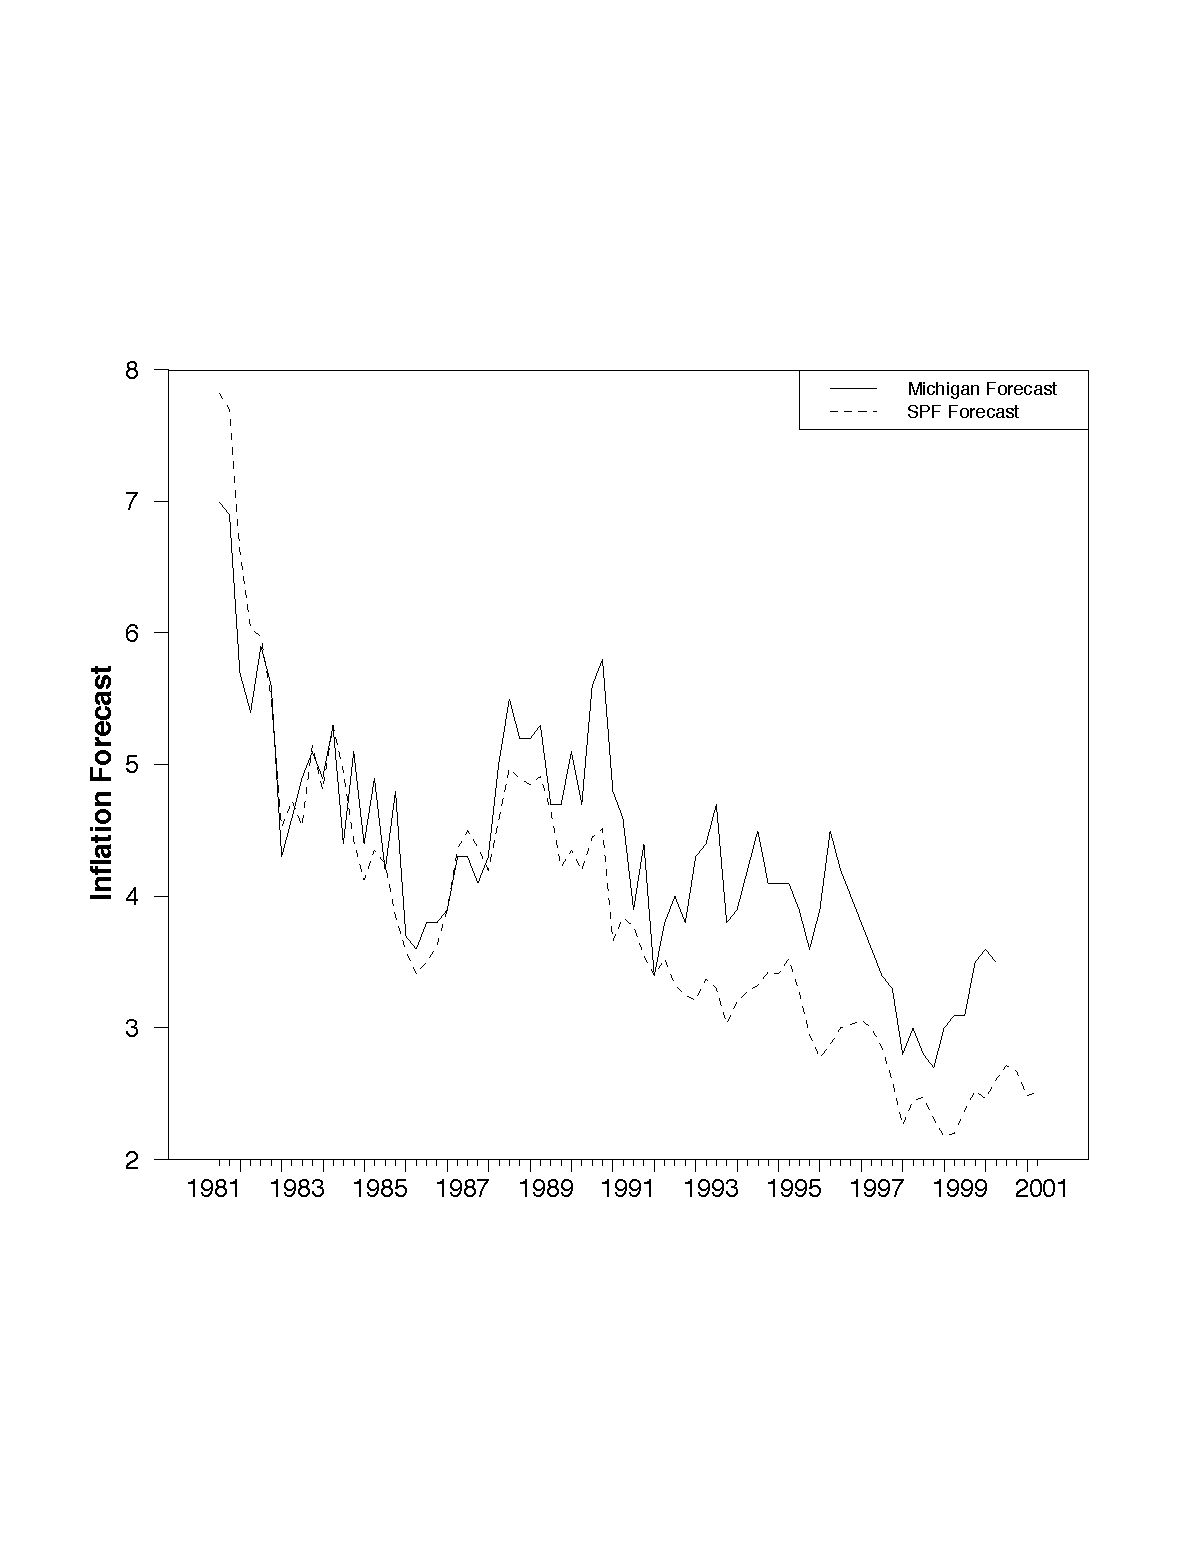
\includegraphics[scale=0.7]{DataAndPrograms/Volumes/Data/inflmicvsspf.eps}}%\epsfbox{DataAndPrograms/Volumes/Data/inflindex.eps}} \caption{Michigan Versus SPF Forecasts of Inflation} \label{fig:inflmicvsspf}\end{figure}

The bottom panel of Figure~\ref{fig:inflfigs} plots the SPF and 
Michigan forecasts since the third quarter of 1981 when the SPF first 
began to include CPI inflation.  One striking feature of the figure is 
that during the high-news-coverage period of the early 1980s, the size 
of the gap between the SPF forecast and the Michigan forecast is 
distinctly smaller than the gap in the later period when there was 
less news coverage of inflation.

A formal statistical test of whether greater news coverage is 
associated with `more rational' household forecasts (in the sense of 
forecasts that are closer to the SPF forecast) can be constructed as 
follows.  Defining the square of the gap between the Michigan and SPF 
forecasts as GAPSQ$_{t} = (M_{t}-S_{t})^{2}$, and defining the 
inflation index as NEWS$_{t}$, we can estimate the simple OLS 
regression equation
\begin{eqnarray}
\mbox{GAPSQ}_{t} & = & \alpha_{0} + \alpha_{1} \mbox{NEWS}_{t}
\end{eqnarray}

Table~\ref{table:erronnews} presents the results.  Estimated over the 
entire sample from 1981q3 to 2000q2 the regression finds a negative 
relationship that is statistically significant at the 5 percent level 
after correcting for serial correlation.  The second row shows that 
that if the first year of the SPF CPI forecasts is excluded the 
negative relationship is much stronger and statistically significant 
at better than the 1 percent level; however, aside from the 
possibility that the first few SPF CPI forecasts were problematic in 
some undetermined way, there seems to be little reason to exclude the 
first year of SPF data.

\input DataAndPrograms/Volumes/Data/erronnews.tex

The finding that household inflation forecasts are better when there 
is more news coverage is an indirect implication of the model under 
the assumption that `infection' is more likely when there is more 
coverage.  The proposition that the infection rate is higher when 
there are more news stories can also be tested directly.  
Table~\ref{table:newslam} presents estimation results comparing the 
infection rate estimated during periods when there is more news 
coverage than average (NEWS$_{t}>$mean(NEWS)) and less coverage than 
average (NEWS$_{t}<$mean(NEWS)).  The estimate of the infection rate 
is almost 0.7 during periods of intensive news coverage, but only 
about 0.2 during periods of less intense coverage; an F-test indicates that 
this difference in coefficients is statistically significant at the 5 
percent level (and nearly at the 1 percent level).

\input DataAndPrograms/Volumes/Data/newslam.tex

There are two strands of the existing literature that deserve comment 
at this point.  In two important recent papers, Akerlof, Dickens, and 
Perry~\cite{adp:one,adp:two} have proposed a model in which workers do 
not bother to inform themselves about the inflation rate unless 
inflation gets high enough that ignorance would become costly.  Since 
periods of high news coverage have coincided with periods of high 
inflation, this model is obviously consistent with the finding that 
mean inflation expectations are more rational during periods of high 
coverage.  Indeed, in a way the ADP models are deeper than the one 
proposed here, because they provide an explanation for the intensity of 
news coverage which is taken as exogenous here: The news media write 
more stories on inflation in periods when workers are more interested 
in the topic.

These results can also be viewed as somewhat similar to some findings 
by Roberts~\cite{roberts:inflexp}, who estimates a model 
like~\eqref{eq:esteqn}, performs a sample split, and finds the speed 
of adjustment parameter much larger in the post-1976 period than in 
the pre-76 era.  He interprets this as bad news for the model.  
However, the pre-76 era was one of much more stable inflation (until 
the last years) than the post-76 era, so the finding of a higher 
coefficient in the later years is very much in the spirit of the tests 
performed above, and is therefore consistent with the epidemiological 
interpretation of the model proposed here.


\section{Unemployment Expectations}

If the epidemiological model of expectations is to be generally useful 
to macroeconomists, it will need to apply to other variables in 
addition to inflation.  Another potential candidate is unemployment 
expectations; in previous work (Carroll~\cite{carroll:brookings}, 
Carroll and Dunn~\cite{carroll&dunn:macroannual}) I have found 
unemployment expectations to be a powerful predictor of household 
spending decisions, and since household spending accounts for two 
thirds of GDP, understanding the dynamics of unemployment expectations 
(and any deviations from rationality) should have considerable direct 
interest.

Unfortunately, however, the Michigan survey's question on unemployment 
does not ask households to name a specific figure for the future 
unemployment rate; instead, households are asked whether they expect 
the unemployment rate to rise, stay the same, or fall over the next 
year.  Traditionally, the answers to these questions are converted 
into an index by subtracting the ``fall'' from the ``rise'' 
proportion.  This diffusion index can then be converted into a 
forecast of the change in the unemployment rate by using the predicted 
value from a regression of the actual change in unemployment on the 
predicted change.

That is, the regression
\begin{eqnarray}
\bar{U}_{t,t+4}-\bar{U}_{t-4,t} & = & \gamma_{0} + \gamma_{1}M_{t}^{U} \label{eq:duonmichu}
\end{eqnarray}
is estimated, where $\bar{U}_{t,t+4}$ is the average unemployment rate 
over the next year and $\bar{U}_{t-4,t}$ is the unemployment rate over 
the year to the present, and $M_{t}^{U}$ is the Michigan index of 
unemployment expectations.  With the estimated 
$\{\hat{\gamma}_{0},\hat{\gamma}_{1}\}$ in hand a forecast of next 
year's inflation rate can be constructed from
\begin{eqnarray}
\hat{\bar{U}}_{t,t+4} & = & \hat{\gamma}_{0} + \hat{\gamma}_{1}M_{t}^{U}+\bar{U}_{t-4,t}.
\end{eqnarray}

When~\eqref{eq:duonmichu} is estimated, the coefficient on $M_{t}^{U}$ 
is has a t-statistic of over 8, even after correcting for serial 
correlation.  However, in a horserace regression of the actual change 
in unemployment on the Michigan diffusion index and the SPF forecast 
of the change in unemployment, the Michigan forecast has no predictive 
power.  Thus, as with inflation, it appears that on average people 
have considerable information about how the unemployment rate is 
likely to change, but forecasters know a lot more than households do.

Table~\ref{table:esteqnunemp} presents a set of regression results for 
the household unemployment forecast that is essentially identical to 
the tests performed in Table~\ref{table:esteqn} for inflation 
expectations.

\input DataAndPrograms/Volumes/Data/esteqn_unemp.tex

The point estimate of the speed of adjustment parameter in row 3 is 
$\alpha_{1}=0.31$; the test reported in the last column of that row 
indicates that this is statistically indistinguishable from the 
estimate of $\lambda=0.25$ obtained for inflation expectations.  In 
most respects, in fact, the epidemiological model performs even better 
in explaining unemployment expectations than explaining inflation 
expectations.  For example, row 3 indicates that the equation does not 
particularly want a constant term in it, while row 4 finds that 
the lagged level of the unemployment rate has no predictive power for 
current expectations even when a constant is excluded.

Nonetheless, this evidence should be considered with some caution.  
The process of constructing the forecast for the average future level 
of the unemployment rate, while apparently reasonable, may be 
econometrically and conceptually problematic.  In particular, this 
method assumes that the {\it amount} by which unemployment is expected 
to change on average is related to the proportion of people who expect 
unemployment to rise or fall; in fact, there is no necessary linear 
relationship between these two quantities.  Other econometric 
difficulties may come from the use of constructed variables on both 
the left and right hand sides of the equation.  I view this model of 
unemployment expectations merely as secondary supporting evidence for 
the expectations modeling strategy pursued here, and therefore am not 
inclined to pursue these conceptual and econometric problems further, 
though they might be worth pursuing in later work.

Other extensions are also possible.  The Michigan survey contains 
questions about future income, interest rates, and other important 
macro variables.  In addition, another monthly survey of consumers 
conducted by the Conference Board has a wide variety of other 
forward-looking questions.  It would be interesting to see whether the 
epidemiological model of expectations is broadly applicable, with a 
parameter value of around 0.25, for many of these variables.


\section{Agent Based Models of Inflation Expectations}

One of the most fruitful trends in empirical macroeconomics over the 
last fifteen years has been the growing effort to construct 
microfoundations that can be tested by examining microeconomic data.  
Broadly speaking, the goal is to find empirically sensible models for 
the behavior of the individual agents (people, firms, banks), which 
can then be aggregated to derive implications about macroeconomic 
dynamics.  Separately, but in a similar spirit, researchers at the 
Santa Fe Institute, the CSED, and elsewhere have been exploring 
`agent-based' models that examine the complex behavior that can 
sometimes emerge from the interactions between collections of simple 
agents.

One of the primary attractions of an agent-based or microfoundations 
approach to modeling household expectations is the prospect of being 
able to test the model using large microeconomic datasets.  However, 
to my knowledge only two existing research papers have examined the 
raw household-level survey data underlying the University of 
Michigan's aggregate expectations index, both by Nicholas 
Souleles~\cite{souleles:sentiment,souleles:finance}.  For present 
purposes, the more interesting of these is 
Souleles~\cite{souleles:sentiment}, which demonstrates (among other 
things) that there are highly statistically significant differences 
across demographic groups in forecasts of aggregate economic variables 
like the inflation rate.  Clearly, in a world where everyone's 
expectations were purely rational, there should be no demographic 
differences in expectations about the inflation rate.

An agent-based version of the framework proposed above could in 
principle account for such demographic differences.  The simplest 
approach would be to assume that there are differences across 
demographic groups in the propensity to pay attention to economic news 
(different $\lambda$'s); it is even conceivable that one could 
calibrate these differences using existing facts about the 
demographics of newspaper readership (or CNBC viewership).

Without access to the underlying micro data it is difficult to tell 
whether demographic heterogeneity in $\lambda$ would be enough to 
explain Souleles's findings about systematic demographic differences 
in macro expectations.  Even without the raw micro data, however, an 
agent-based model has considerable utility.  In particular, an 
agent-based approach permits us to examine the consequences of 
relaxing some of the model's assumptions to see how robust its 
predictions are.  Given our hypothesis that Souleles's results on 
demographic differences in expectations might be due to differences in 
$\lambda$ across groups, the most important application of the 
agent-based approach is to determining the consequences of 
heterogeneity in $\lambda$.

\subsection{Heterogeneity in $\lambda$}

Consider a model in which there are two categories of people, each of 
which makes up half the population, but with different 
newspaper-reading propensities, $\lambda_{1}$ and $\lambda_{2}$.

For each group it will be possible to derive an equation like 
\eqref{eq:esteqn},
\begin{eqnarray}
 M_{i,t}[\pi_{t,t+4}] & = & \lambda_{i} N_{t}[\pi_{t,t+4}] + (1-\lambda_{i}) M_{i,t-1}[\pi_{t-1,t+3}].
\end{eqnarray}

But note that (dropping the $\pi$ arguments for simplicity) aggregate 
expectations will just be the population-weighted sum of expectations 
for each group,
\begin{eqnarray}
   M_{t} & = & (M_{1,t} + M_{2,t})/2
\\ & = & \left(\frac{\lambda_{1}+\lambda_{2}}{2}\right)N_{t} + ((1-\lambda_{1})M_{1,t-1}+(1-\lambda_{2})M_{2,t-1})/2
\end{eqnarray}

Replace $M_{1,t-1}$ by $M_{t-1} + (M_{1,t-1}-M_{t-1} )$ and 
similarly for $M_{2,t-1}$ to obtain
\begin{eqnarray}
 M_{t} & = & \left(\frac{\lambda_{1}+\lambda_{2}}{2}\right) N_{t} + \left(1-\left(\frac{\lambda_{1}+\lambda_{2}}{2}\right)\right)M_{t-1}+\overbrace{\left(\frac{M_{1,t-1}+M_{2,t-1}}{2}\right)-M_{t-1}}^{=0} \nonumber
\\ & & -  \left(\frac{\lambda_{1} (M_{1,t-1}-M_{t-1})+\lambda_{2} (M_{2,t-1}-M_{t-1})}{2}\right)
\\ M_{t} & = & \hat{\lambda} N_{t} + (1-\hat{\lambda}) M_{t-1} - \left(\frac{\lambda_{1} (M_{1,t-1}-M_{t-1})+\lambda_{2} (M_{2,t-1}-M_{t-1})}{2}\right) \label{eq:lambda12}
\label{eq:heterolam}
\end{eqnarray}
where $\hat{\lambda} = (\lambda_{1}+\lambda_{2})/2$.

Thus, the dynamics of aggregate inflation expectations with 
heterogeneity in $\lambda$ have a component $\hat{\lambda} 
N_{t}+(1-\hat{\lambda}) M_{t-1}$ that behaves just like a version of 
the model when everybody has the same $\lambda$ equal to the average 
value in the population, plus a term (in big parentheses in 
\eqref{eq:lambda12}) that depends on the joint distribution of 
$\lambda$'s and the deviation by group of the difference between the 
previous period's rational forecast and the group's forecast.

Now consider estimating the baseline equation
\begin{eqnarray}
        M_{t} & = & \lambda N_{t}+ (1-\lambda) M_{t-1} \label{eq:base}
\end{eqnarray}
on a population with heterogeneous $\lambda$'s.  The coefficient 
estimates will be biased in a way that depends on the correlations of 
$N_{t}$, $M_{t-1}$ and $M_{t}$ with the last term in 
equation~\eqref{eq:heterolam}, $\left(\frac{\lambda_{1} 
(M_{1,t-1}-M_{t-1})+\lambda_{2} (M_{2,t-1}-M_{t-1})}{2}\right)$.  
There is no analytical way to determine the magnitude or nature of the 
bias without making a specific assumption about the time series 
process for $N_{t}$, and even with such an assumption all that could 
be obtained is an expected asymptotic bias.  The bias in any 
particular small sample would depend on the specific history of 
$N_{t}$ in that sample.

The only sensible way to evaluate whether the bias problem is likely 
to be large given the actual history of inflation and inflation 
forecasts in the US is to simulate a model with households who have 
heterogeneous $\lambda$'s and to estimate the baseline equation on 
aggregate statistics generated by that sample.

Specifically, the experiment is as follows.  A population of $P$ 
agents is created, indexed by $i$; each of them begins by drawing a 
value of $\lambda_{i}$ from a uniform distribution on the interval 
$(\underline{\lambda},\overline{\lambda})$.  In an initial period $0$, 
each agent is endowed with an initial value of $M_{i,0}$ = 2 percent.  
Thus the population mean value $M_{0}= (1/P) \sum_{i=1}^{P} M_{i,0} = 
2$.  For period $1$, each agent draws a random variable distributed on 
the interval $[0,1]$.  If that draw is less than or equal to 
the agent's $\lambda_{i}$, the agent updates $M_{i,1} = N_{1}$ where $N_{1}$ 
is taken to be the `Newspaper' forecast of the next year's inflation 
rate in period $t$; if the random draw is less than $\lambda_{i}$ the 
agent's $M_{i,1} = M_{i,0}$.  The population-average value of $M_{1}$ 
is calculated, and the simulation then proceeds to the next period.

For the simulations, the `news' series $N_{t}$ is chosen as the 
concatenation of 1) the actual inflation rate from 1960q1 to 1981q2 
and 2) the SPF forecast of inflation from 1981q3 to 2001q2.  Then 
regression equations corresponding to~\eqref{eq:base} are estimated on 
the subsample corresponding to the empirical subsample, 1981q3 to 
2001q2.  Thus, the simulation results should indicate the dynamics of 
$M_{t}$ that would have been observed if actual newspaper forecasts of 
inflation had been a random walk until 1981q2 and then had tracked the 
SPF once the SPF data began to be published.

The results of estimating~\eqref{eq:esteqn} on the data generated by 
this simulation when the population is $P=250,000$ are presented in 
Table~\ref{table:estonsim}.  For comparison, and to verify that the 
simulation programs are working properly, equation (1) presents 
results when all agents' $\lambda$'s are exogenously set to 0.25.  As 
expected, the simulation returns an estimate of $\lambda = 0.25$, and 
the equation fits so precisely that there are essentially no 
residuals.

\begin{table}
\input DataAndPrograms/Volumes/Data/estonsim.tex
\end{table}


The remaining rows of the table present the results in the case where 
$\lambda$ values are heterogeneous in the population.  The second row 
presents the most extreme example, 
$[\underline{\lambda},\overline{\lambda}] = [0.00,0.50]$.  
Fortunately, even in this extreme case the regression yields an 
estimate of the speed-of-adjustment parameter $\lambda$ that, at 
around $0.26$, is still quite close to the true average value $0.25$ 
in the population.  Interestingly, however, one consequence of the 
heterogeneity in $\lambda$ is that there is now a very large amount of 
serial correlation in the residuals of the equation; the Durbin-Watson 
statistic indicates that this serial correlation is postive and a Q 
test shows it to be highly statistically significant.

Heterogeneous $\lambda$'s induce serial correlation primarily because 
the views of people with $\lambda$'s below $\bar{\lambda}$ are slow to 
change.  For example, if the `rational' forecast is highly serially 
correlated, an agent with a $\lambda$ close to zero will be expected 
to make errors of the same size and direction for many periods in a 
row before finally updating.

The comparison of the high serial correlation that emerges from this 
simulation to the low serial correlation that emerged in the empirical 
estimation in Table~\ref{table:esteqn} suggests that heterogeneity in 
$\lambda$ is probably not as great as the assumed uniform distribution 
between 0.0 and 0.5.  Results are therefore presented for a third 
experiment, in which $\lambda$'s are uniformly distributed between 0.2 
and 0.3.  Estimation on the simulated data from this experiment yields 
an estimate of $\lambda$ very close to 0.25 and a Durbin-Watson 
statistic that indicates much less serial correlation than emerged 
with the broad $[0,0.5]$ range of possible $\lambda$'s.  Finally, the 
last row presents results when $\lambda$ is uniformly distributed over 
the interval [0.15,0.35].  This case is intermediate: the estimate of 
$\lambda$ is still close to 0.25, but the Durbin-Watson statistic now 
begins to indicate substantial serial correlation.

On the whole, the simulation results suggest that the serial 
correlation properties of the empirical data are consistent with a 
moderate degree of heterogeneity in $\lambda$, but not with extreme 
heterogeneity.  It is important to point out, however, that empirical 
data contain a degree of measurement and sampling error that is absent 
in the simulated data.  To the extent that these sources can be 
thought of as white noise, they should bias the Durbin-Watson 
statistic up in comparison to the `true' Durbin-Watson, so the scope 
for heterogeneity in $\lambda$ is probably considerably larger than 
would be indicated by a simple comparison of the measured and 
simulated Durbin-Watson statistics.  Thus the serial correlation 
results should not be taken as very serious evidence against 
substantial heterogeneity in $\lambda$.

A few last words on serial correlation.  The important point in Mankiw 
and Reis~\cite{mankiw&reis:stickye}, as well as in work by 
Ball~\cite{ball:nearrational} and others, is that the presence of some 
people whose expectations are not fully and instantaneously 
forward-looking profoundly changes the behavior of macro models.  
Thus, the discussion of serial correlation has an importance here 
beyond its usual econometric ramifications for standard errors and 
inference.  If there are some consumers whose expectations are very 
slow to update, they may be primarily responsible for important 
deviations between the rational expectations model and macroeconomic 
reality.


\subsection{Matching the Standard Deviation of Inflation Expectations}

Thus far all our tests of the model have been based on its predictions 
for behavior of mean inflation expectations.  Of course, the model 
also generates predictions for other statistics like the standard 
deviation of expectations across households at a point in time.  Some 
households will have expectations that correspond to the most recent 
inflation forecast, while others will have expectations that are out 
of date by varying amounts.  One prediction of the model is that (for 
a constant $\lambda$) if SPF inflation forecasts have remained stable 
for a long time, the standard deviation of expectations across 
households should be low, while if there have been substantial recent 
changes in the rational forecast of inflation we should expect to see 
more cross-section variability in households' expectations.

This is testable.  Curtin~\cite{curtin:inflsurvart} reports average 
values for the standard deviation for the Michigan survey's inflation 
expectations over the period from 1978 to 1995; results are plotted as 
the solid line in figure~\ref{fig:inflstd}.  It is true that the 
empirical standard deviation was higher in the early 1980s, a time 
when inflation rates and SPF inflation expectations changed rapidly 
over the course of a few years, than later when the inflation rate was 
lower and more stable.

\input DataAndPrograms/Volumes/Data/inflstd.tex
% This figure is generated in the estonsim (or AgentSocialSim) program

%\begin{figure} \centerline{\includegraphics[scale=0.6]{DataAndPrograms/Volumes/Data/inflstdsim.eps}}%\epsfbox{DataAndPrograms/Volumes/Data/inflindex.eps}} \caption{Standard Deviation of Inflation Expectations from Michigan Survey} \label{fig:inflstdsim}\end{figure}

The short and long dashed loci in the figure depict the predictions 
of the homogeneous $\lambda=0.25$ and heterogeneous $\lambda \in 
[0.0,0.5]$ versions of the agent-based model.  There is considerable 
similarity between the time paths of the actual and simulated standard 
deviations: The standard deviation is greatest for both simulated and 
actual data in the late 1970s and early 1980s, because that is the 
period when the levels of both actual and expected inflation changed 
the most.  In both simulated and real data the standard deviation 
falls gradually over time, but shows an uptick around the 1990 
recession and recovery before returning to its downward path.

However, the {\it levels} of the standard deviations are very 
different between the simulations and the data; the scale for the 
Michigan data on the right axis ranges from 4 to 11, while the scale 
for the simulated standard deviations on the left axis ranges from 0 
to 3.  Over the entire sample period, the standard deviation of 
household inflation expectations is about 6.5 in the real data, 
compared to only about 0.5 in the simulated data.

Curtin~\cite{curtin:inflsurvart} analyzes the sources of the large 
standard deviation in inflation expectations across households.  He 
finds that part of the extreme variability is attributable to small 
numbers of households with very extreme views of inflation.  Curtin's 
interpretation is that these households are probably just 
ill-informed, and he proposes a variety of other ways to extract the 
data's central tendency that are intended to be robust to the presence 
of these extreme outlying households.  However, even Curtin's 
preferred measure of dispersion in inflation expectations, the size of 
the range from the 25th to the 75th percentile in expectations, has an 
average span of almost 5 percentage points over the 81q3-95q4 period, 
much greater than would be produced by any of the simulation models 
considered above.\footnote{Curtin advocates use of the median rather 
than the mean as the summary statistic for `typical' inflation 
expectations.  However, the epidemiological model has simple 
analytical predictions for the mean but not the median of household 
expectations, so the empirical work in this paper uses the mean.}

The first observation to make about the extreme variability of 
household inflation expectations is that such variability calls into 
question almost all standard models of wage setting in which 
well-informed workers demand nominal wage increases in line with a 
rational expectation about the future inflation rate.\footnote{The 
only prominent exception I am aware of is the two papers by Akerlof, 
Dickens, and Perry~\cite{adp:first,adp:second} mentioned briefly above.  In 
these models workers do not bother to learn about the inflation rate 
unless it is sufficiently high to make the research worthwhile.  
However such a model would presumably imply a modest upper bound to 
inflation expectation errors, since people who suspected the inflation 
rate was very high would have the incentive to learn the truth.  In 
fact, Curtin (1996) finds that the most problematic feature of the 
empirical data is the small number of households with wildly 
implausibly high forecasts.} If a large fraction of workers have views 
about the future inflation rate that are a long way from rational, it 
is hard to believe that those views have much impact on the 
wage-setting process.  Perhaps it is possible to construct a model in 
which equilibrium is determined by average inflation expectations, 
with individual variations making little or no no difference to 
individual wages.  Constructing such a model is beyond the scope of 
this paper; but whether or not such a model is proposed, it seems 
likely that any thorough understanding of the relation between 
inflation expectations in the aggregate and actual inflation will need 
a model of how individuals' inflation expectations are determined.

The simplest method of generating extra individual variability in 
expectations is to assume that when people encounter a news report on 
inflation, the process of committing the associated inflation forecast 
to memory is error-prone.\footnote{ Alternatively, one could assume 
that retrieval from memory is error-prone.  The implications are very 
similar but not identical.}

\input DataAndPrograms/Volumes/Data/inflstdlogerr.tex
% This figure is generated in the estonsim or AgentSocialSim program


To be specific, suppose that whenever an agent encounters a news report 
and updates his expectations, the actual expectation stored in memory 
is given by the expectation printed in the news report times a 
mean-one lognormally distributed storage error.  Since the errors 
average out in the population as a whole, this assumption generates 
dynamics of aggregate inflation expectations that are identical to 
those of the baseline model.  Figure~\ref{fig:inflstdlogerr} plots the 
predictions for the standard deviation of inflation expectations 
across households of the baseline $\lambda=0.25$ model with a 
lognormally distributed error with a standard error of 0.5.  The 
figure shows that the change in the standard deviation of inflation 
residuals over time is very similar in the model and in the data, but 
the level of the standard deviation is still considerably smaller in 
the model.  This could of course be rectified by including an additive 
error in addition to the multiplicative error.  Such a proposed 
solution could be tested by examining more detailed information on the 
structure of expectations at the household level like that examined by 
Souleles~\cite{souleles:sentiment}.

\subsection{Social Transmission of Inflation Expectations}

As noted above, the standard model of disease transmission is one in 
which illness is transmitted by person-to-person contact.  
Analogously, it is likely that some people's views about inflation are 
formed by conversations with others rather than by direct contact with 
news reports.  For the purposes of this paper the most important 
question is whether the simple formula~\eqref{eq:esteqn} would do a 
reasonably good job in capturing the dynamics of inflation 
expectations even when social transmission occurs.

Simulation of an agent-based model with both modes of transmission is 
straightforward.  The extended model works as follows.  In each period, 
every person has a probability $\lambda$ of obtaining the latest 
forecast by reading a news story.  Among the $(1-\lambda)$ who do not 
encounter the news source, the algorithm is as follows.  For each 
person $i$, there is some probability $p$ that he will have a 
conversation about inflation with a randomly-selected other person $j$ 
in the population.  If $j$ has an inflation forecast that is of more 
recent vintage than $i$'s forecast, then $i$ adopts $j$'s forecast, 
and vice-versa.\footnote{This rules out the possibility that the 
less-recent forecast would be adopted by the person with a more-recent 
information.  The reason to rule this out is that if there were no 
directional bias (more recent forecasts push out older ones), the 
swapping of information would not change the distribution of forecasts 
in the population and therefore would not result in aggregate dynamics 
any different from those when no social communication is allowed.}

\input DataAndPrograms/Volumes/Data/estran.tex


Table~\ref{table:estran} presents results of estimating 
equation~\eqref{eq:esteqn} on the aggregate inflation expectations 
data that result from this agent-based simulation under a uniform 
fixed $\lambda=0.25$ probability of news-reading.  The first two rows 
present results when the probability of a social transmission event is 
$p=0.25$.  The primary effect of social transmission is to bias upward 
the estimated speed of adjustment term.  The point estimate is about 
0.31, or about 6 percentage points too high.  However, the $\bar{R}^2$ 
of the equation is virtually 100 percent, indicating that even when 
there is social transmission of information, the common-source model 
does an excellent job of explaining the dynamics of aggregate 
expectations.  The next row shows the results when the rate of social 
transmission is $p=0.10$.  Unsurprisingly, the size of the bias in the 
estimate of $\lambda$ is substantially smaller in this case, and the 
model continues to perform well in an $\bar{R}^{2}$ sense.

A potential objection to these simulations is that they assume `random 
mixing.'  That is, every member of the population is equally likely to 
encounter any other member.  Much of the literature on agent-based 
models has examined the behavior of populations that are distributed 
over a landscape in which most interactions occur between adjacent 
locations on the landscape.  Often models with local but no global 
interaction yield quite different outcomes from `random mixing' 
models.

To explore a model in which social communication occurs locally but 
not globally, I constructed a population distributed over a two 
dimensional lattice, of size 500x500, with one agent at each lattice 
point.  I assumed that a fraction $\eta$ of agents are `well 
informed' - that is, as soon as a new inflation forecast is released, 
these agents learn the new forecast with zero lag.  Other agents in 
the population obtain their views of inflation solely through 
interaction with neighbors.\footnote{For the purposes of the 
simulation, an agent's neighbors are the agents in the eight cells 
surrounding him.  For agents at the borders of the grid, neighborhoods 
are assumed to wrap around to the opposite side of the grid; 
implicitly this assumes the agents live on a torus.} Thus, in this 
model, news travels out in concentric patterns (one step on the 
landscape per period) from its geographical origination points (the 
news agents, who are scattered randomly across the landscape).  As in 
the random mixing model, I assume that new news drives out old news.

\input DataAndPrograms/Volumes/Data/estnbr.tex

Results from estimating the baseline model on data produced by the 
`local interactions' simulations are presented in 
table~\ref{table:estnbr}.  For comparability with the baseline 
estimate of $\lambda=0.25$ in the common-source model, I have assumed 
that proportion $\eta=0.25$ of the agents in the new model are the 
`well-informed' types whose inflationary expectations are always up to 
date.  Interestingly, estimating the baseline model yields a 
coefficient of about $\alpha_{1}=0.22$ on the SPF forecast, even 
though 25 percent of agents always have expectations exactly equal to 
the SPF forecast.  The coefficient on lagged expectations gets a value 
of about 0.71, and the last column indicates that a test of the 
proposition that $\alpha_{1}+\alpha_{2}=1$ now rejects strongly.  
However, the regression still has an $\bar{R}^{2}$ of around 0.99, so 
the basic common-source model still does an excellent job of capturing 
the dynamics of aggregate inflation expectations.

The most interesting result, however, is shown in the next row: The 
estimation now finds a highly statistically significant role for a 
nonnegligible constant term.  Recall that the only real empirical 
problem with the common-source model was that the estimation found a 
statistically significant role for a constant term.

Results in the next rows show what happens when the proportion of news 
agents is reduced to $\eta = 0.15$.  As expected, the estimate of 
$\alpha_{1}$ falls; indeed, the downward bias is now even more 
pronounced than with 25 percent well-informed.  However, when a 
constant is allowed into the equation, the constant term itself is 
highly significant and the estimate of $\alpha_{1}$ jumps to about 
0.18, not far from the fraction of news agents in the population.

What these simulation results suggest is that the empirical constant 
term may somehow be reflecting the fact that some transmission of 
inflation expectations is through social exchange rather than directly 
through the news media.  Furthermore, and happily, it is clear from 
the structure of the local interactions model that this population 
would eventually learn the true correct expectation of inflation if 
the SPF forecasts permanently settled down to a nonstochastic 
steady-state.  Thus it is considerably more appealing to argue that 
the constant term reflects misspecification of the model (by leaving 
out social interactions) than to accept the presence of a true 
constant term (and its associated implication of permanent bias).


It is tempting to view the social learning simulations as a bit of a 
sideshow to the main thrust of this paper, which is about the 
surprisingly good fit of the common source epidemiological model.  
However, it is worth repeating the central lesson of Mankiw and 
Reis~\cite{mankiw&reis:stickye} and others: The extent to which 
inflation can be reduced without increasing unemployment depends upon 
the speed with which a new view of inflation can be communicated to 
the {\it entire} population.  It is not at all clear that the 
predictions about the medium-term inflation/unemployment tradeoff of a 
model with social transmission of expectations, or even of the 
common-source model with heterogeneous $\lambda$'s, are similar to the 
predictions of the homogeneous $\lambda$ model examined by Mankiw and 
Reis~\cite{mankiw&reis:stickye}.  Investigating these questions should
be an interesting project for future research.


\section{Conclusions}

This paper has three main points.  

The first is that it is past time, more than 25 years after the
`rational expectations revolution' and 65 years after Keynes's
emphasis on the centrality of expectations, that the examination of
empirical data on expectations became a central part of
macroeconomics.  While there have been a few important prior
contributions (particularly by
Roberts~\cite{roberts:stickyinfl,roberts:inflexp}), and a modest
literature on consumer sentiment and consumption expenditures (see,
e.g., Carroll, Fuhrer, and Wilcox~\cite{cfwSentiment}), the bulk of the
macroeconomics profession has ignored the rich empirical data
available on actual household and business expectations in favor of
the theoretical appeal of rational expectations models.

The second point is that the abandonment of rational expectations need
not lead macroeconomics into an atheoretical wilderness where the
Lucas critique lurks behind every equation.  There is an existing body
of theory, in epidemiology as well as in the `small worlds'
literature, that can be directly applied to explain expectations
formation.  This paper has shown that for inflation expectations and
unemployment expectations, a remarkably simple epidemiological model
does an excellent job in explaining the deviations of mean household
expectations from a rational forecast.

The final point is that if we want to have macroeconomic models that
are built on really secure microfoundations, and are therefore as
immune as can reasonably be hoped from the Lucas critique, there is no
substitute for building the model from the ground up, and comparing
its predictions to whatever microeconomic data are available.  Whether
the enterprise is described as a search for the `microfoundations' of
macroeconomics or as `agent-based' modeling, it seems reasonable to
suppose that in the long run no macro model will be counted on as a
reliable guide to macro behavior if its predictions for the
expectations of individual actors bear little empirical resemblance to
the observable expectations of actual individuals.


\vfill\eject

\input /Software/latex/texhtml


\pagebreak\vfill\eject
\appendix


\centerline{\large Appendix A: Timing Issues}
\medskip\medskip\medskip

This appendix explores implications of the very different sampling
methodologies of the Michigan household survey and the Survey of 
Professional Forecasters.  

As noted in the main text, timing issues suggest that when estimating
the model with monthly data the timing problems are least serious 
when the sample is restricted to months $t$ in which a Survey of 
Professional Forecasters was conducted and published.  The 
appropriate estimating equation in this case is 
\begin{eqnarray}
M_{t+1}[\pi_{t+1,t+13}] & = & \lambda N_{t}[\pi_{t,t+12}] + (1-\lambda) M_{t}[\pi_{t,t+12}].
\end{eqnarray}

However, there is a problem in estimating this equation directly.  The 
monthly Michigan data reflect surveys of only 500 households, and the 
estimated sampling error with such a small sample is no longer trivial 
enough to be ignored.  Fortunately, Curtin~\cite{curtin:inflsurvart} has 
provided estimates of the magnitude of the sampling error.  Curtin's 
results imply a typical sampling variance of about 0.09 per month, 
large enough to cause substantial bias in our estimate of $\lambda$ if 
not corrected for.  Fortunately, standard econometric formulas can be 
used to adjust parameter estimates when the variance of the sampling 
error is known.  

The corrected point estimate of the speed-of-adjustment parameter is 
$1-\lambda=0.91$.\footnote{The programs, dataset, and econometric 
derivations that generate this result are included in the downloadable 
files associated with this paper on my website; the econometric 
theory, and derivation of the estimated sampling variance of 0.09, are 
laid out in \texttt{AppendixA\_MonthlyExp.pdf}, the RATS program that 
estimates the model is \texttt{AppendiA\_MonthlyExp.pgm}, and the 
documentation of the program is in 
\texttt{AppendixA\_MonthlyPgm.pdf}.} Reassuringly, this estimate is 
right in the ballpark of what would have been expected if there were 
no data or reporting difficulties in the quarterly estimation 
procedure: The quarterly estimation of the baseline model produced a 
quarterly updating fraction of $(1-\lambda)=0.73$, which is 
statistically indistinguishable from the estimate of $0.92^{3} \approx 
0.78$ implied by the fact that a quarter contains three months.  Thus, 
the procedure of estimating the model with the appropriate monthly 
data, being careful about measurement error, yields essentially the 
same answer as was obtained from quarterly data.

The preceding analysis glosses over a final problem: The Michigan 
survey data are collected on a continous basis throughout a month, 
rather than all at once on the first day of the month.  To see why 
this is potentially problematic, consider again a month $t$ in which 
an SPF survey is conducted.  Since inflation statistics are reported 
in mid-month, roughly half of the households surveyed in month $t$ 
will have had the opportunity to read the news articles published upon 
the release of the statistics at mid-month, while the other half will 
not.  In this case I have not been able to derive a `clean' equation 
like \eqref{eq:monthlym3} for the dynamics of inflation expectations.

To investigate the importance of this problem, I conducted the 
following simulation analysis.  First, I specified a daily-frequency 
stochastic process for the `rational' forecast of the next year's 
inflation as a random walk with a daily innovation such that the 
quarterly innovations in the inflation forecast would match the 
standard deviation of the actual quarterly innovations in the SPF 
forecast.  I assumed that households update to this true forecast 
using a $\lambda$ parameter such that $(1-\lambda)^{n} = 0.75$ where 
$n$ is the number of days in a quarter.  I then picked out the value
of the `rational' forecast at the midpoint of each quarter, and 
set a variable equal to that forecast.  Finally, I aggregated the
daily data to quarterly frequency, and performed a regression of
the form
\[
M_{t} = \lambda S_{t} + (1-\lambda) M_{t-1}
\]
where $M_{t}$ now represents the quarterly average of the simulated 
daily values of the constructed household forecast and $S_{t}$ is the 
value of the `true' forecast at the midpoint of the quarter.  This 
exercise produced an estimated $\lambda=0.234$ as compared with the 
`correct' $\lambda=0.25$.  Thus, it appears that the mismatch in 
timing between the Michigan and SPF surveys is unlikely to cause much 
of a problem in estimating the $\lambda$ parameter.\footnote{These 
simulations are conducted by the program 
\texttt{AppendixA\_TimingSims.pgm}.}

\pagebreak\vfill\eject

\centerline{\Large Appendix B: Construction of Index of News Coverage}
\medskip\medskip\medskip

The index of news stories on inflation was constructed as follows.  
For each newspaper $i \in \{\mbox{New York Times},\mbox{Washington 
Post}\}$, for each year $t$ since 1980 (when the Nexis index of both 
newspapers begins), a search was performed for stories that began on 
the front page of the newspaper and contained words beginning with the 
root `inflation' (so that, for example, `inflationary' or 
`inflation-fighting' would be picked up).

For each newspaper, the number of stories was converted to an index 
ranging between zero and 1 by dividing the number of stories in a 
given year by the maximumn number of inflation stories in any year.  
Thus, the fact that the overall index falls to about 0.25 in the last 
part of the sample indicates that there were about a quarter as many 
front-page stories about inflation in this time period as there were 
at the maximum.

\pagebreak\vfill\eject

\bibliographystyle{/Software/latex/econometrica_fullnames}
\bibliography{/Software/latex/economics}



\end{document}
\pagebreak\vfill\eject

\input DataAndPrograms/Volumes/Data/adfpi.tex
\input DataAndPrograms/Volumes/Data/piforc.tex
\input DataAndPrograms/Volumes/Data/esteqn.tex
\input DataAndPrograms/Volumes/Data/erronnews.tex
\input DataAndPrograms/Volumes/Data/newslam.tex
\input DataAndPrograms/Volumes/Data/esteqn_unemp.tex
\input DataAndPrograms/Volumes/Data/estonsim.tex

\input DataAndPrograms/Volumes/Data/inflfigs.tex
\input DataAndPrograms/Volumes/Data/inflstd.tex
\input DataAndPrograms/Volumes/Data/inflstdlogerr.tex




The ancient Greek philosopher Xenophanes once observed that if oxen 
had artistic talent, the gods they would paint would look like oxen 
instead of like Apollo or Aphrodite.  

Xenophanes might not have been surprised to learn that the agents with 
whom economists populate their models are essentially godlike versions 
of economists: infinitely knowledgable and infinitely rational and 
deeply interested in the structure and workings of the economy.  
However, in a twist that surely would have surprised even Xenophanes, 
we assume that these godlike creatures are a good representation of 
the average person or business manager.

\begin{eqnarray}
        M_{t}[\pi_{t+1}] & = & \lambda N_{t}[\pi_{t+1}] + (1-\lambda)\lambda E_{t-1}[\pi_{t+1}]+(1-\lambda)^{2} \lambda E_{t-2}[\pi_{t+1}] + \ldots .
\end{eqnarray}
\begin{eqnarray*}
        \pi_{t-4,t} & = & \pi_{t-3}+\pi_{t-2}+\pi_{t-1}+\pi_{t}  \\
         & = & F_{t-3}[\pi_{t-3}]+\epsilon_{t-3}+F_{t-2}[\pi_{t-2}]+\epsilon_{t-2}  
 +F_{t-1}[\pi_{t-1}]+\epsilon_{t-1}+F_{t}[\pi_{t}]+\epsilon_{t}
\\   & = & 4 F_{t-3}[\pi_{t-3}] + 3 \eta_{t-2}+2\eta_{t-1}+\eta_{t}
+ \epsilon_{t-3}+\epsilon_{t-2}+\epsilon_{t-1}+\epsilon_{t}
\end{eqnarray*}
and analogously 
\begin{eqnarray*}
        \pi_{t,t+4} & = & 4 F_{t+1}[\pi_{t+1}]  + 3 \eta_{t+2}+2\eta_{t+3}+\eta_{t}
+ \epsilon_{t+1}+\epsilon_{t+2}+\epsilon_{t+3}+\epsilon_{t+4}
\\ & = & 4 F_{t-3}[\pi_{t-3}]+4(\eta_{t-2}+\eta_{t-1}+\eta_{t}+\eta_{t+1})+ 3 \eta_{t+2}+2\eta_{t+3}+\eta_{t}
\\ &   & + \epsilon_{t+1}+\epsilon_{t+2}+\epsilon_{t+3}+\epsilon_{t+4}
\end{eqnarray*}

Consider how 
the inflation rate



If inflation is indeed a unit root process with a white noise 
transitory component, then the inflation rate over the next 
year will be
\begin{eqnarray*}
        \pi_{t,t+4} & = & F_{t}[\pi_{t+1}]+\epsilon_{t+1}+F_{t+2}[\pi_{t+2}]+\epsilon_{t+2}
+ F_{t+3}[\pi_{t+3}]+\epsilon_{t+3}+F_{t+4}[\pi_{t+4}]+\epsilon_{t+4}   
\\       & = & 4 F_{t}[\pi_{t}]+4\eta_{t+1}+3 \eta_{t+2}+2\eta_{t+3}+\eta_{t+1}+\epsilon_{t+1}+\epsilon_{t+2}+\epsilon_{t+3}+\epsilon_{t+4}
%\\      & = & F_{t}[\pi_{t-1,t}]+\chi_{t,t+4}
\end{eqnarray*}
where 
$E_{t}[\eta_{t+1}]=E_{t}[\eta_{t+2}]=E_{t}[\epsilon_{t+1}]=E_{t}[\epsilon_{t+2}]=\ldots=0$ 
implies that $\chi_{t,t+4}$ is a white noise error term.  That is, the 
only element of predictability in future inflation rates comes from 
the fact that the future fundamental rate is equal to the current 
fundamental rate plus some white noise innovations.




Now consider a regression
of the inflation rate over the next year on the inflation rate for the
current quarter:
\begin{eqnarray}
        \pi_{t,t+4} & = & \alpha_{0}+\alpha_{1} \pi_{t-1,t}
\\  F_{t}[\pi_{t-1,t}]+\chi_{t,t+4}             & = & \alpha_{0}+\alpha_{1} (F_{t}[\pi_{t-1,t}]+\epsilon_{t})
\\  F_{t}[\pi_{t-1,t}]                  & = & \alpha_{0}+\alpha_{1} (F_{t}[\pi_{t-1,t}]+\epsilon_{t})-\chi_{t,t+4}
\end{eqnarray}

If the variance of the transitory component of inflation were zero, 
the regression should 


 then the only 
predictable element of the difference between inflation over the next 
year and inflation in the current quarter would come from the 
$-4\epsilon_{t}$ term.  

Table~\ref{table:survforecast} presents evidence on these questions.  
The first two rows show that both the Michigan inflation expectations 
index and the SPF forecast have highly statistically significant 
predictive power for the core inflation rate, even when the lagged 
core inflation rate is included as a regressor; indeed, in neither 
case is the lagged inflation rate statistically significant, which 
indicates that both survey measures already incorporate any 
information contained in the lagged inflation rate.\footnote{The 
Durbin-Watson and Q statistics indicate that there is a substantial 
amount of serial correlation in the residuals from these equations, so 
the standard errors are adjusted using the Newey-West correction with 
8 lags and a damping factor of 1.}$^{,}$\footnote{It might seem that 
this evidence that the Michigan index can forecast the change in the 
inflation rate contradicts the assumption that people believe 
inflation follows a random walk.  In fact, however, there is no 
contradiction.  In our model, people believe that future 
fundamental inflation rates follow a random walk beginning in period 
$t+1$.  But their views of the inflation rate for period $t+1$ are not 
constrained to be a random innovation with respect to the actual 
inflation rate in period $t$, for two reasons.  First, we assumed that 
people in period $t$ believe that $F_{t}[\pi_{t+1}]$ is equal to 
the rational forecast $E_{t}[\pi_{t+1}]$, and there is no restriction 
on how the rational forecast may differ from the recent level of 
inflation; in particular, the rational forecast may be influenced, for 
example, by the level of the unemployment rate.  Second, people in 
this model know that any transitory inflation shocks in period $t$ 
will disappear for future periods.} The third row of the table shows 
that when both survey measures are included in the forecasting 
equation, the Michigan survey measure has no information about the 
future inflation rate that is not contained in the SPF forecast, while 
the SPF forecast has considerable and highly statistically significant 
predictive power not contained in the Michigan forecast.  The SPF's 
victory is made more impressive by the fact that the SPF forecast is 
constructed in the middle of the second month of the quarter, and 
therefore by construction cannot incorporate any information released 
during the latter half of the quarter, while the Michigan survey 
measure for the corresponding quarter includes results from interviews 
up to the last day of the quarter.  The fact that the SPF contains 
considerably more forecasting power despite its substantial timing 
disadvantage bolsters the proposition that the SPF forecast is 
considerably better than the Michigan forecast.

An alternative way to examine the rationality and efficiency of the 
two forecasts is to ask about the ability of the two surveys to 
forecast the {\it change} in the inflation rate.  In a statistical 
sense this can be viewed as a tougher challenge than forecasting the 
level of the inflation rate; after all, if the inflation rate really 
has a unit root (which we could not reject above), then the level of 
the inflation rate would be highly forecastable but changes in the 
inflation rate (beyond the current quarter) would be totally 
unforecastable.  The next three panels of the table therefore regress 
the change in the annual inflation rate between the present and one 
year in the future on the SPF and Michigan survey's forecasts of that 
change.  That is, 

\begin{eqnarray*}
        \pi_{t-4,t} & = & \pi_{t-3}+\pi_{t-2}+\pi_{t-1}+\pi_{t}  \\
         & = & F_{t-3}[\pi_{t-3}]+F_{t-2}[\pi_{t-2}]+F_{t-1}[\pi_{t-1}]+F_{t}[\pi_{t}]  \\
         &  & + \epsilon_{t-3}+\epsilon_{t-2}+\epsilon_{t-1}+\epsilon_{t}
\end{eqnarray*}

\begin{eqnarray*}
        F_{t}[\pi_{t,t+4}] & = & 4 F_{t}[\pi_{t+1}]
\end{eqnarray*}

Comparing these two expressions, it is evident that there are 
several

Again, both surveys contain highly statistically significant 
information, but again the SPF forecast is substantially better than 
the Michigan forecast.\footnote{In principle, such predictability 
could reflect either time aggregation problems or the modest 
predictability that comes from knowing that the current transitory 
components of inflation will disappear.  The }


Now we can integrate the fact that experts have some ability to 
predict the future inflation rate with the person's view that the 
inflation process has a unit root by supposing that when people 
update their views about the fundamental inflation rate they update to 
what they perceive to be the fully-rational forecast of the 
fundamental rate.



  
That is, if we denote the fully-rational forecast of next quarter's 
inflation rate as $E_{t}[\pi_{t+1}]$, people who are updating their 
forecasts in quarter $t$ set
\begin{eqnarray}
        F_{t}[\pi_{t,t+1}] & = & E_{t}[\pi_{t,t+4}].
\end{eqnarray}



This assumption can be justified by noting that newspaper articles on 
inflation almost invariably incorporate interviews with economists who 
are experts on forecasting the inflation rate.  While the news event 
that triggers the article is likely to have been the release of the 
latest inflation statistics, the job of a good journalist is to 
provide perspective and to extract the meaning of those statistics, 
which is done largely through interviews with experts.  Furthermore, 
an examination ofa sample of these articles indicates that the most 
common form of forecast is for the inflation rate over the next year; 
it is rare for expert forecasts of any particular future quarter to 
appear.  It is not implausible, therefore, to suppose that at least 
part of what readers take away from such stories is a sense of what to 
expect for the average inflation rate over the next year, which (under 
people's views of the inflation process) should be the same as the 
inflation forecast for the next quarter.

people's belief in a unit root in the inflation process implies that
\begin{eqnarray}
        F_{t}[\pi_{t+2}] & = & F_{t}[\pi_{t+1}] 
\\  F_{t}[\pi_{t+3}] & = & F_{t}[\pi_{t+2}] = F_{t}[\pi_{t+1}]  
\end{eqnarray}
and so on.

% Consider putting in the fact that the SPF forecast of the quarterly
% inflation rate has a mean absolute change of 0.3 from tp1 to tp4,
% and 0.2 from tp2 to tp4.  This shows that a constant F is not
% implausible


At this point it will be useful to introduce some simplifying 
notation.  Denote the inflation rate (expressed at an annual rate) 
between period $t$ and period $t+n$ as $\pi_{t,t+n}$.  Thus what we 
have previously written as $\pi_{t+1}$ becomes $4 \pi_{t,t+1}$, where 
the 4 is required to convert the quarterly rate to an annual rate and 
the subscripts indicate that inflation is measured as the change in 
the log price level between period $t$ and $t+1$.  Using this 
notation, \eqref{eq:with4} can be rewritten:
\begin{eqnarray}
        M_{t}[\pi_{t,t+4}] & = & \lambda E_{t}[\pi_{t,t+1}]+(1-\lambda) M_{t-1}[\pi_{t-1,t+3}] . \label{eq:esteqn}
\end{eqnarray}


because the quarterly data we have used 
for the Michigan inflation forecast and the SPF forecast do not map 
very well into our model.


This would suggest 
that if month $t$ is an SPF survey month news reports from that month


If we suppose that news reports on inflation continue to reflect fresh 
contacts between reporters and the participants in the SPF between SPF 
reporting intervals, then the evolution of news media reports will 
depend on how often the typical forecaster updates his forecast.  The 
simplest case would be if all forecasters' inflation forecasts were 
adjusted only once per quarter, just prior to the collection of the 
SPF data.  In this case we could expect newspaper reports to reflect 
the latest SPF forecast all the way up to the point where the new SPF 
forecast is collected.  

I have been unable to find systematic information about how often most 
forecasters' forecasts are updated.  The one forecaster whose methods 
are a matter of public record is the Federal Reserve, whose entire 
macroeconomic forecast is updated roughly once every six weeks (to 
coincide with the monetary policy meetings of the Federal Open Market 
Committee).  If other forecasters were on a similar schedule we would 
expect a given SPF forecast to provide an accurate picture of actual 
forecasts only for about 1-1/2 quarters.


To discuss this question clearly we need to introduce a notational 
convention about the monthly value to be assumed for the SPF forecast 
in months for which no SPF forecast is collected.  Define an operator 
$S_{t}[\pi_{t,t+12}]$ which returns the value of the SPF forecast

If we denote the SPF forecast collected in month $t$ as 
$S_{t}[\pi_{t,t+12}]$.

then this assumption would imply that the 
newspaper reports would be captured by
\begin{eqnarray}
    N_{t+1}[\pi_{t+1,t+13}] & = & S_{t}[\pi_{t,t+12}]
\\  N_{t+2}[\pi_{t+2,t+14}] & = & S_{t}[\pi_{t,t+12}]
\\  N_{t+3}[\pi_{t+3,t+15}] & = & S_{t}[\pi_{t,t+12}]
\end{eqnarray}
where the timing is dictated by the fact that the SPF data are not 
published until near end of the month so that it only becomes possible 
for them to be published in news reports beginning in the next month.  
The second and third equations indicate same SPF forecast continues to 
be published until a new forecast is available.


To discuss this question clearly we need to introduce a notational 
convention about the monthly value to be assumed for the SPF forecast 
in months for which no SPF forecast is collected.  Define an operator 
$S_{t}[\pi_{t,t+12}]$ which returns the value of the SPF forecast

If we denote the SPF forecast collected in month $t$ as 
$S_{t}[\pi_{t,t+12}]$.

then this assumption would imply that the 
newspaper reports would be captured by
\begin{eqnarray}
    N_{t+1}[\pi_{t+1,t+13}] & = & S_{t}[\pi_{t,t+12}]
\\  N_{t+2}[\pi_{t+2,t+14}] & = & S_{t}[\pi_{t,t+12}]
\\  N_{t+3}[\pi_{t+3,t+15}] & = & S_{t}[\pi_{t,t+12}]
\end{eqnarray}
where the timing is dictated by the fact that the SPF data are not 
published until near end of the month so that it only becomes possible 
for them to be published in news reports beginning in the next month.  
The second and third equations indicate same SPF forecast continues to 
be published until a new forecast is available.





The simplest assumption we could make about the news media's inflation 
reporting would be that journalists simply look up the latest 
published forecast from the SPF when they compose their news reports.  
This assumption can be criticized on several grounds.  The first is 
that real journalists like to quote individual forecasters rather than 
reprint results of a publicly available survey; it seems plausible, 
therefore, that the news reports about inflation that are printed 
between the middle and the end of a month in which the survey is taken 
will on average reflect the forecasts made by the survey participants 
in that month, because the journalists are probably contacting roughly 
the same people as were contacted by the SPF. Since most inflation 
articles are published shortly after release of the month's inflation 
data and the articles often reflect interviews asking forecasters how 
the latest data affect their inflation outlook, it seems likely that 
most of the inflation articles published in a survey month will 
actually incorporate the information that is subsequently published in 
the SPF. This would imply that if month $t$ is a survey month,
\begin{eqnarray}
    N_{t}[\pi_{t,t+12}] & = & S_{t}[\pi_{t,t+12}]
\\  N_{t+1}[\pi_{t+1,t+13}] & = & S_{t}[\pi_{t,t+12}]
\\  N_{t+2}[\pi_{t+2,t+14}] & = & S_{t}[\pi_{t,t+12}]
\end{eqnarray}

The assumption that news reports keep repeating the last SPF forecast 
until a new one is collected is also questionable.  If forecasters 
update their forecasts more frequently than the SPF data are 
collected, newspaper reports on inflation are likely to reflect this 
new information in the period before the next SPF forecast is 
conducted.  However, in the absence of survey data in the intervening 
months, little can be done about this problem except to note that it 
may introduce some specification error that makes fit of the equation 
deteriorate.

Furthermore, while there 
is typically only a single rational expectations solution to a macro 
model, dropping any element of the rational expectations framework 
often leads to a model with many possible equilibria which are 
difficult to choose among.

Furthermore, it seems 
likely that a rigorous model of calculation-cost-minimization would 
lead to a periodic (`time dependent') solution rather than 
probabilistic updating.

If month $t$ happened to be a month in which a SPF survey was 
conducted, it seems likely that 


No similar equation would apply for month $t+2$ or $t+3$ because the
SPF forecast is collected only every third month.  Even if people


Consider first the SPF forecasts.  On the other hand, m

Assuming that the professional forecasters whom the 
journalists interview for their stories are able to process the new 
inflation data quickly, it seems likely that the news stories on 
inflation in mid-month will reflect mostly the same forecasts that are 
later reported in the SPF.

However, by the time month $t+2$ ends the SPF forecast is more than 
two and a half months out of date.  There will have been two new 
statistical reports about both inflation and unemployment, income, 
retail sales, and capacity utilization that have arrived.  Assuming 
that news reports through the end of month $t+2$ continue to reflect 
the same forecast that was collected in the middle of month $t$ seems 
inappropriate.  The situation is even worse for the first half of 
month $t+3$, because there will have been three reports on 
unemployment, income, and retail sales since the last SPF forecasts 
were collected.  The safest course would seem to be to estimate
\eqref{eq:monthlym3} only on data from months that were the final
month in a quarter, where the model can most realistically be said
to apply.


One way to investigate this is through a simulation analysis in which 
the process for $N_{t}$ is taken to be the actual time path of SPF 
forecasts, and we assume that $\lambda_{1}= 0.15$ while $\lambda_{2} = 
0.35$, yielding an {\it average} infection rate of 0.25.  Results of 
estimating~\eqref{eq:base} on this population are presented in 
Table~\ref{table:estonsim}.  Fortunately, the point estimate is quite 
close to 0.25, which suggests that when there is heterogeneity in 
$\lambda$, estimation of our baseline model will return a $\lambda$ 
that is close to the mean $\lambda$ in the population.

The final row of the table presents results from an intermediate case 
where the $\lambda$'s are heterogeneous within a restricted range from 
$\lambda = 0.2$ to $\lambda = 0.3$.  Again the estimate of $\lambda$ 
is very close to its population mean, but the Durbin-Watson statistic 
indicates that correlation consequences of $\lambda$ heterogeneity are 
much more modest.


Inflation 
expectations were chosen as the primary modeling target for two 
reasons.  First, standard theories of inflation imply that workers' 
inflation expectations can importantly influence inflation outcomes: 
Workers who expect higher inflation should push for greater wage 
increases, pushing up employers' costs and therefore prices.  Second, 
inflation expectations are one of the few macroeconomic variables for 
which a long time series exists on the expectations of the typical 
household.  The expectations data come from the University of 
Michigan's monthly Survey of Consumers, which is also the source for 
the closely-watched consumer sentiment index.  The baseline version of 
the model generates a simple analytical expression for the evolution 
of expectations that can be estimated using the published Michigan 
data.  The model turns out to do a remarkably good job in explaining 
these data, yielding an estimate that at any given time only about a 
quarter of households have fully up-to-date inflation expectations.


If not, the most fruitful direction to explore 
next would probably be whether the literature on `small world' social 
networks could be applied to the problem.  (The small world literature 
examines the patterns of connection and transmission of information 
among members of social networks that exhibit both local 
(neighborhood) and global connections.  See 
Watts~\cite{watts:smallworld} for an excellent overview.)

The primary conclusion is that the baseline equation for the model 
without social communication does a very good job in capturing the 
aggregate dynamics of inflation expectations even when social 
communication exists.  However, the estimate of the 
speed-of-transmission parameter $\lambda$ is biased upward, because 
news now spreads faster through the population than in the baseline 
model.

